\documentclass[10pt]{article}
%\documentclass[10pt]{book}

\usepackage[draft]{fixme}

\usepackage{listings}
\usepackage{html}
\usepackage{color}
\usepackage{multicol}
\usepackage{multirow}
\usepackage{graphicx}
\usepackage{alltt}
% style for code listing
\lstset{language={C},basicstyle=\scriptsize} 
\newcommand{\hlstd}[1]{\textcolor[rgb]{0,0,0}{#1}}
\newcommand{\hlkey}[1]{\textcolor[rgb]{0,0,0}{\bf{#1}}}
\newcommand{\hlnum}[1]{\textcolor[rgb]{0.16,0.16,1}{#1}}
\newcommand{\hltyp}[1]{\textcolor[rgb]{0.51,0,0}{#1}}
\newcommand{\hlesc}[1]{\textcolor[rgb]{1,0,1}{#1}}
\newcommand{\hlstr}[1]{\textcolor[rgb]{1,0,0}{#1}}
\newcommand{\hldstr}[1]{\textcolor[rgb]{0.51,0.51,0}{#1}}
\newcommand{\hlcom}[1]{\textcolor[rgb]{0.51,0.51,0.51}{\it{#1}}}
\newcommand{\hldir}[1]{\textcolor[rgb]{0,0.51,0}{#1}}
\newcommand{\hlsym}[1]{\textcolor[rgb]{0,0,0}{#1}}
\newcommand{\hlline}[1]{\textcolor[rgb]{0.33,0.33,0.33}{#1}}

\newcommand{\mySmallFontSize}{\scriptsize}
\newcommand{\mySmallestFontSize}{\tiny}

\newcommand{\codeFontSize}{\scriptsize}
\newcommand{\code}[1]{{\scriptsize #1}}

% Software version number
%\newcommand{\VersionNumber}{@VERSION@}

%\newcommand{\ExampleDirectory}{@top_srcdir@/projects/compass/tests}

% Latex trick to allow us to comment out large sections of documentation
\newcommand{\commentout}[1]{}

% change the title of the Fixme List
\renewcommand{\listfixmename}{Things to Fix in Documentation}

\newcommand{\comm}[2]{\bigskip
                      \begin{tabular}{|p{11cm}|}\hline
                      \multicolumn{1}{|c|}{{\bf Comment by #1}}\\ \hline
                      #2\\ \hline
                      \end{tabular}
                      \bigskip
                     }

\def\verbatimfile#1{\begingroup
                    \@verbatim \frenchspacing \@vobeyspaces
                    \input#1 \endgroup
}

\newcounter{lineno}

% Taken from verbatimfiles.sty on web
\makeatletter %JCL

\def\verbatimlisting#1{\setcounter{lineno}{0}%
    \begingroup \@verbatim \frenchspacing \@vobeyspaces \parindent=20pt
    \everypar{\stepcounter{lineno}\llap{\thelineno\ \ }}\input#1
    \endgroup
}

\makeatother %JCL

% \endinput

\addtolength{\textheight}{0.5in}
\sloppy

%---------------------------------------------------------------------
% Begin Document
%---------------------------------------------------------------------

\begin{document}

% This draft mode eliminates the figures (leaves boxes for where they would be)
%\textcolor{green}{(Associated with ROSE Version @VERSION@)} } }
%\psdraft

\title{ {\bf \textcolor{red}{A ROSE-Based End-to-End Empirical Tuning
  System for Whole Applications} \\ 
              \textcolor{blue}{Draft User Tutorial} \\
%              \textcolor{green}{(Associated with ROSE Version @VERSION@)} 
              } }
\author{ {\bf Chunhua Liao and Dan Quinlan} \\
         Lawrence Livermore National Laboratory \\ 
         Livermore, CA  94550 \\
         925-423-2668 (office)  925-422-6278 (fax) \\
         \{liao6, quinlan1\}@llnl.gov \\
         Project Web Page:
         \htmladdnormallink{http://www.rosecompiler.org}{http://www.rosecompiler.org} \\
         UCRL Number for ROSE User Manual: UCRL-SM-210137-DRAFT \\
         UCRL Number for ROSE Tutorial: UCRL-SM-210032-DRAFT \\
         UCRL Number for ROSE Source Code: UCRL-CODE-155962 \\ \\
         \htmladdnormallink{ROSE User Manual
         (pdf)}{http://www.rosecompiler.org/ROSE_UserManual/ROSE-UserManual.pdf} \\
         \htmladdnormallink{ROSE Tutorial
         (pdf)}{http://www.rosecompiler.org/ROSE_Tutorial/ROSE-Tutorial.pdf} \\
         \htmladdnormallink{ROSE HTML Reference (html
         only)}{http://www.rosecompiler.org/ROSE_HTML_Reference/index.html}
       }
\maketitle
\newpage


% This fixes the really long table of contents problem
\setcounter{tocdepth}{2}

\tableofcontents
\newpage
%

\chapter{ Introduction }

\label{introduction:introduction}

% Purpose:
%\begin{itemize}
%   \item A. Section overview
%   \item B. Why you should read this manual
%   \item C. How to use this manual
%   \item D. Terminology
%   \item E. Overview of library
%   \item F. Program control
%   \item G. Error messages
%   \item H. Section summary
%\end{itemize}
%\begin{center}
%*********************  \newline
%\end{center}
%\vspace{0.25in}

% Quote:
% The successful con artist is a mirror of the time and place where he works.

%\textcolor{red}{ROSE}

% Include common text used in both the manual and the tutorial
\section{What is ROSE}

% Describe ROSE to the broad target audience.
% Describe how it works 
%    Read the input source code
%    Generate the AST (define AST and define graph) 
%       The structure of the original source code is preserved
%       Details aboaut the source code can be found in the AST
%    Provide tools 
%       for the analysis and transformation of the AST
%       generate additional information from the AST (call graph, etc.)
%       visualization of the program
%    Source code regeneration
%
   ROSE is an open source compiler infrastructure for building tools that can
read and write source code in multiple languages (C/C++/Fortran) and/or analyze
binary executables (using the x86, Power-PC, and ARM instruction sets).
The target audience for ROSE is people building tools for the analysis
and transformation of software generally as well as code generation tools.
% source code and/or analysis of binary executables.
ROSE provides a library (librose) that can be 
used to support the universal requirements of tools that
do custom analysis and/or transformations on source code
and custom analysis of binary forms of software. ROSE is 
portable across and expanding range of operating systems
and work with an growing number of compilers.

   ROSE provides a common level of infrastructure support to
user-defined tools, so that they need not implement the 
complex support required for software analysis and transformation operations. 
For source code based tools these include parsing, common forms of 
compiler analysis, common transformations, and code generation.
For binary analysis based tools these include disassembly,
function boundary detection, and common forms of analysis.
User defined tools may also mix source code and binary analysis
to form more interesting tools for specialized purposes.
ROSE is part of research work to unify the analysis of
both source code and binaries within general compiler research
and define mixed forms of static and dynamic analysis.

   ROSE works by reading the source code and/or binary
and generating an Abstract Syntax Tree (AST).  The AST forms
a graph representing the structure of the source code and/or binary
executable and is held in memory to provide the fastest possible means 
of operating on the graph.  The nodes used to define the AST graph are 
an {\em intermediate representation} (IR); common within compiler research
as a way of representing the structure of software absent syntax details
(commas, semi-colons, white-space, etc.).  ROSE provides mechanisms to 
traverse and manipulate the AST. Finally, in the case of source code, 
ROSE provides mechanisms to regenerate source code from the AST.

   As a trivial example, if the input source code program contains a variable declaration
for an integer, all of this information will be available in the AST generated from
the input code passed on the command line to any tool built using ROSE.
Similarly, an automated transformation of the variable declaration 
held in the AST would be expressed using a traversal over the AST and
code {\em semantic actions} to mutate the AST. Then the transformed source code would be 
generated ({\em unparsed}) from the AST.  In the case of binaries 
(including executables, object files, and libraries), the AST will 
represent the structure of the binary. The AST for a binary also includes the 
binary file format (symbol table, debug format, import tables, etc.), 
disassembled instructions, all instruction operands, etc.

   ROSE provides a rich set of tools to support the analysis of 
software including the support for users to build their own forms
of analysis and specialized transformations. As an example, ROSE includes
a full OpenMP compiler built using the internal ROSE infrastructure 
for analysis and transformation.
A wide assortment of AST traversals are provided
to express both analysis and transformations of the AST. A set of
common forms of analysis are provided (call graph, control flow, etc.)
most work uniformly on both source code and binary executables.
Visualization support in included to help users understand and debug
their tools.  GUI support is available to support building professional
level tools using ROSE. ROSE is actively supported by a small
group at LLNL and is used as a basis for compiler research work within 
DOE at LLNL.

   Technically, ROSE is designed to build what are called {\em translators}, 
ROSE uses a source-to-source approach to define such translators. Note that 
translators are significantly more sophisticated than {\em preprocessors} 
but the terms are frequently confused. A translator must understand the 
source code at a fundamentally deeper level using a grammar for the whole language
and on the whole source code, where as a preprocessor only understands the 
source code using a simpler grammar and on a subset of the source code. 
It is {\em loosely} the difference between any language compiler and the 
C preprocessor (cpp).

% Sections suggested by Carol Eidt (at Microsoft)
\section{Why you should be interested in ROSE}
ROSE is a tool for building source-to-source translators.
You should be interested in ROSE if you want to 
understand or improve any aspect of your software. ROSE
makes it easy to build tools that read and operate on source code
from large scale applications (millions of lines).  Whole projects
may be analyzed and even optimized using tools built using ROSE.
For example, ROSE is itself analyzed nightly using ROSE.

To get started immediately consult the ROSE User Manual, chapter
{\em Getting Started} for details).

\section{Problems that ROSE can address}
    ROSE is a mechanism to build source-to-source analysis or 
optimization tools that operate directly on the source code of large 
scale applications.  Example tools that {\em have} been built include:
\begin{itemize}
   \item OpenMP translator,
   \item Array class abstraction optimizer,
   \item Source-to-source instrumenter,
   \item Loop analyzer,
   \item Symbolic complexity analyzer,
   \item Inliner and outliner,
   \item Code coverage tools,
   \item and many more...
\end{itemize}
Example tools that {\em can} be built include:
\begin{itemize}
   \item Custom optimization tools,
   \item Custom documentation generators,
   \item Custom analysis tools,
   \item Code pattern recognition tools,
   \item Security analysis tools,
   \item and many more...
\end{itemize}


\section{Research Goals for ROSE}
ROSE is a project that aims to define a new type of compiler technology that allows
compilation techniques to address the optimization of user-defined abstractions.
Due to the nature of the solution we provide, it is also an open compiler infrastructure
that can be used for a wide number of other purposes.

   User-defined abstractions are built from within an existing base language and
carry specific semantic information that can't be communicated to the base
language's compiler.  In many situations, the semantic information could be useful within
program optimization, but the base-language compiler is forced to ignore this semantic 
information because there is no way for applications to pass such additional information 
to the base-language compiler. Note that {\tt \#pragmas} only permit information that the 
base-language compiler might anticipate (expect) to be passed; it is not a meaningful 
mechanism to communicate arbitrary information about user-defined abstractions to a 
compiler.  ROSE is a part of general research on {\em telescoping languages} (a term 
coined by Ken Kennedy at Rice University) and CELL languages (a term coined by 
Bjarne Stroustrup).  It is part of general work to define domain-specific languages
economically from general purpose languages.

\fixme{Check spelling of CELL in recent work by Bjarne}

\section{ROSE: A Tool for Building Source-to-Source Translators}

   ROSE represents a tool for building source-to-source translators.
Such translators can be useful for many purposes:
\begin{itemize}
   \item automated analysis and/or modification of source code
   \item instrumentation
   \item data extraction
   \item building domain-specific tools
\end{itemize}
An optimizing translator can be expected to both analyze the input 
source code and automatically generate transformations of the source code; the
result being a new source code. If successful, the automatically generated source 
code will demonstrate better performance.  ROSE is the tool that helps users write
such source-to-source translators.  Expected users would be library writers and
tool developers, not necessarily the application developers.  As a result, we expect
the ROSE user to be more knowledgeable about programming languages issues than the 
average application developer.

ROSE translators are particularly useful as a way to bridge the gap between what we want
compilers to do and what they actually do.  This {\em semantic gap} is significant when
optimizing user-defined abstractions (functions and/or data structures), because the
base-language compiler has no knowledge of their semantics.  The optimization
is particularly important within scientific applications.  Such applications are often
expensive to build because they are exceedingly complex and must too often be
written at low levels of abstraction to maintain significant performance on
modern computer architectures.  The modern computer architectures themselves also
vary widely and make the optimization of software difficult.

\section{Motivation for ROSE}

   The original motivation for the development of ROSE comes from work within the Overture Project
to develop abstractions for numerical computation that are efficient and easy to use.
Basically, C++ language mechanisms made the abstractions easy to use (if not tedious to
build), but efficiency was more problematic since the optimization of low-level
abstractions can be (and frequently is) not handled well by the compiler.  Specifically
the rich semantic information the library writer embeds into his abstractions can't
be communicated to the compiler, so many optimizations are missed.  ROSE has addressed
this fundamental problem by simplifying how an optimized translator could be built and
tailored to a library's abstractions to introduce optimizations that use the high-level 
semantics of user-defined abstractions.

\section{ROSE as a Compiler Framework}

    ROSE contains compiler infrastructure. This is because a translator that reads
source code in any language is essentially a compiler (or {\em translator}).  The most precise understanding
of a source code in any language is the process of compiling it.  Source-to-source
compilation can, however, skip the common back-end code generation (since source code is
generated instead of object code in the form of an executable).  ROSE translators
pay particular attention to reconstruct the generated source code (including comments and
CPP translator control directives [\#include, \#if, \#else, \#endif, etc.], and 
the original application's indentation and variable names, etc.).

    ROSE is unique because 
% What is different about ROSE is that 
it makes traditional compiler infrastructure
accessible to library and tool developers who are not likely to have a significant compiler
background.  Still, some basic knowledge of an Abstract Syntax Tree (AST) is 
assumed (and, unfortunately, currently required).  
% In future work we will continue to simplify what is presently required background, as much as possible.

   Figure \ref{introduction:phases} shows the different phases of processing within ROSE.

\begin{figure}
%\centerline{\epsfig{file=rose-processing-phases.ps,height=1.0\linewidth,width=1.0\linewidth,angle=0}}

%\centerline{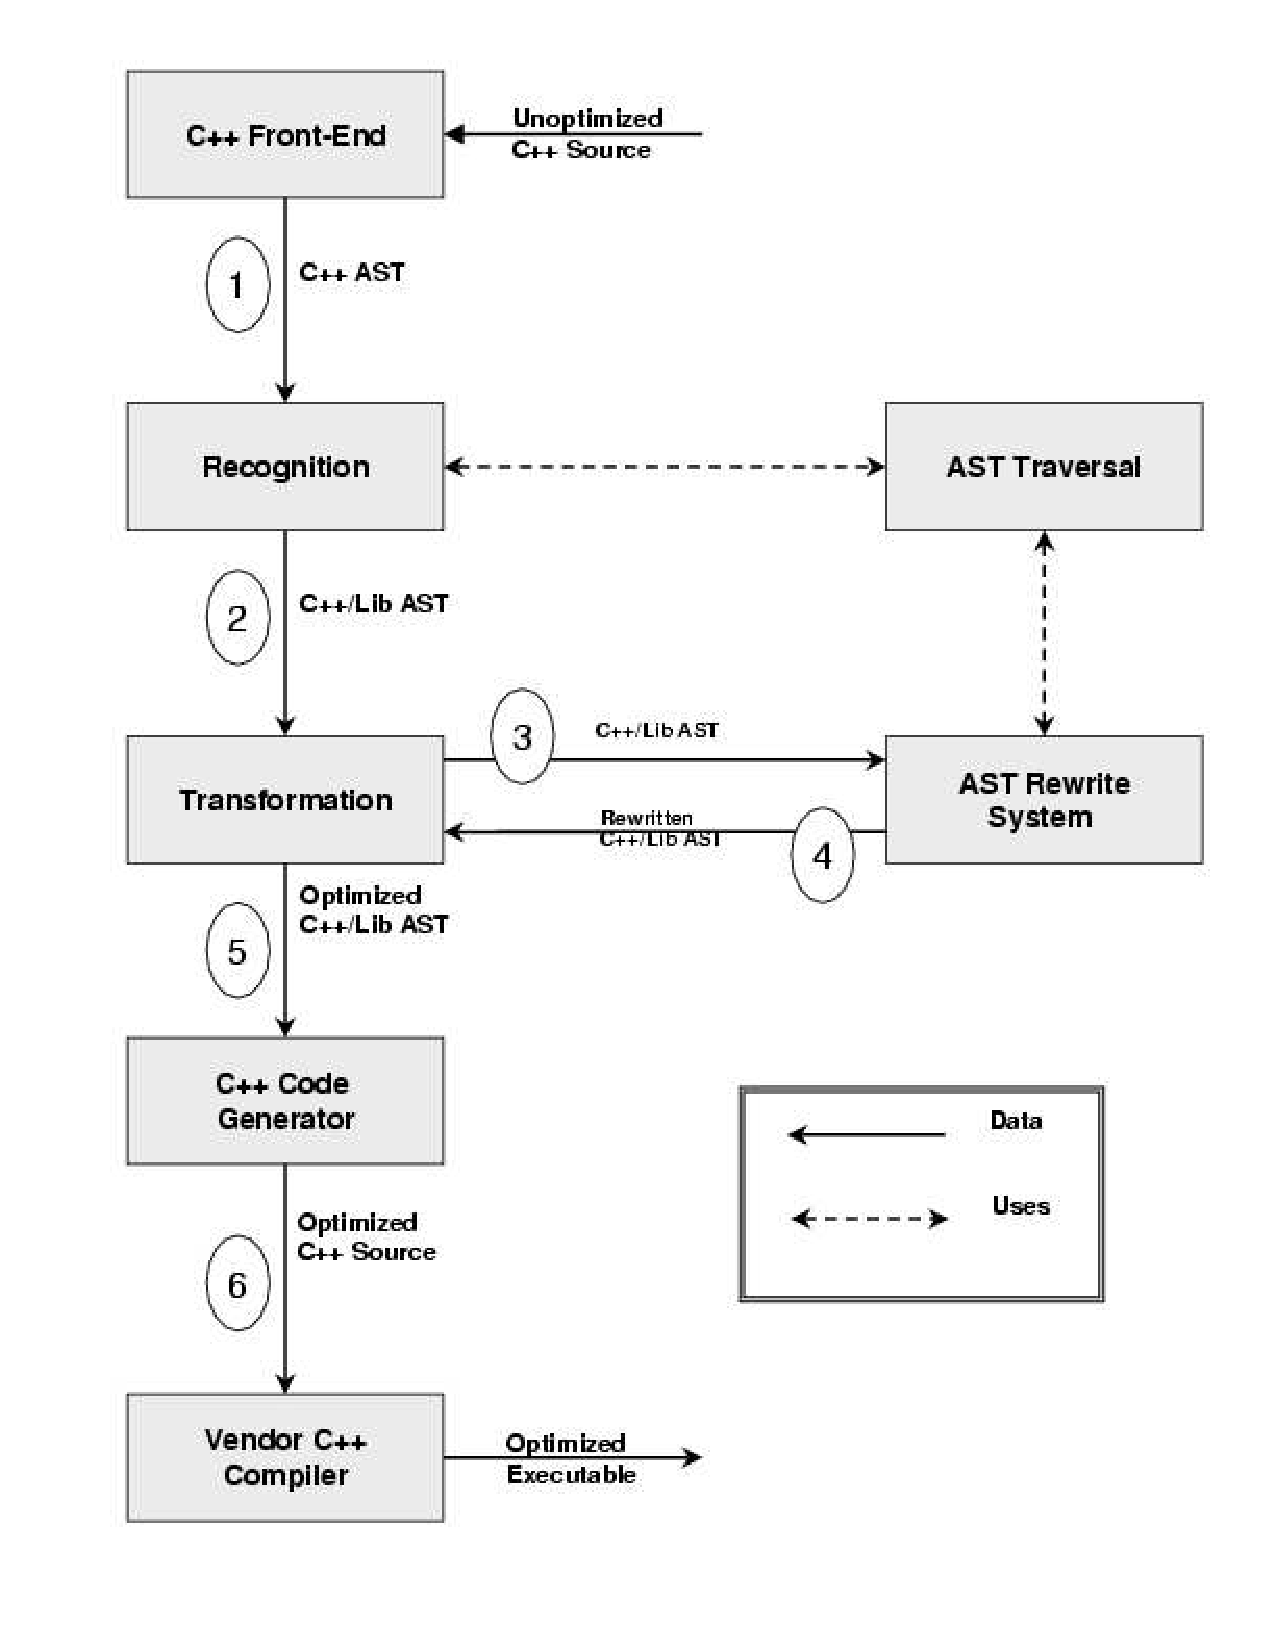
\psfig{file=rose-processing-phases.pdf,height=1.0\linewidth,width=1.0\linewidth,angle=0}}
%\centerline{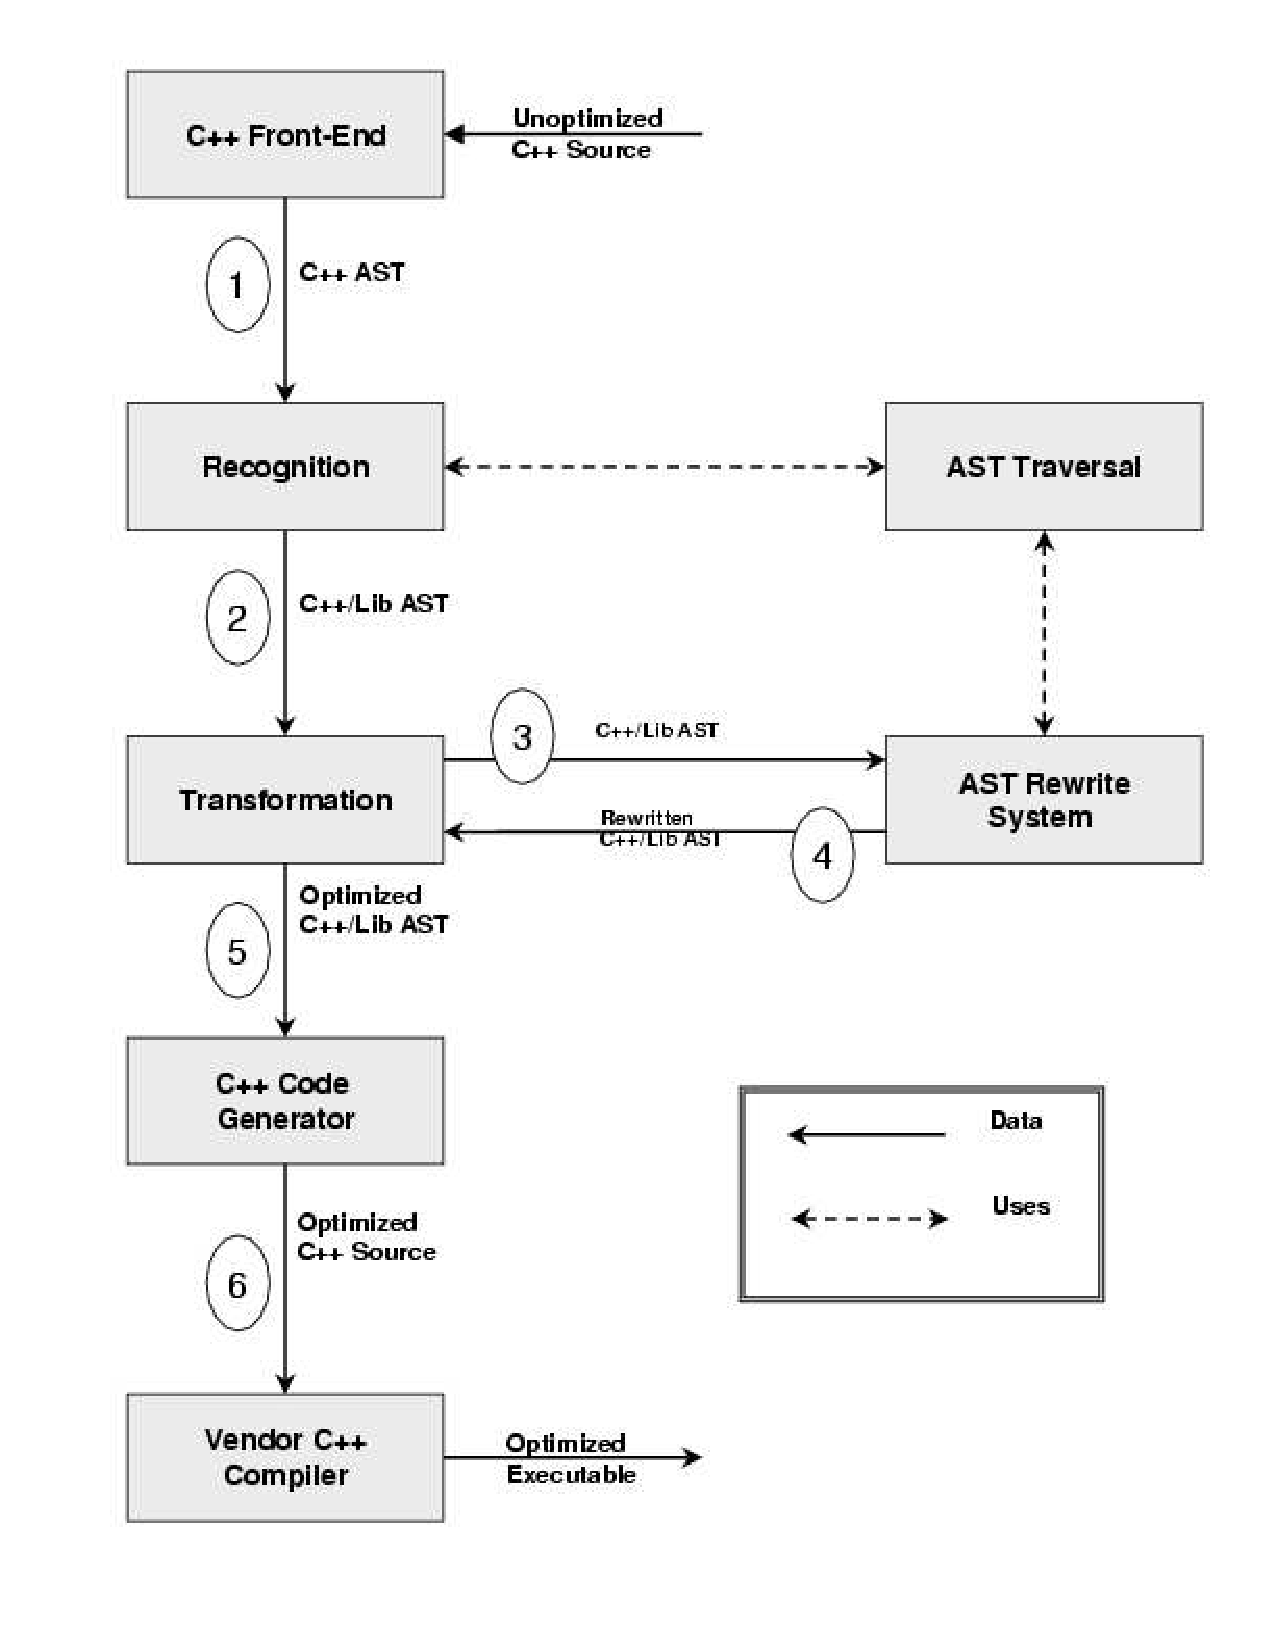
\includegraphics[height=1.0\linewidth,width=1.0\linewidth,angle=0]{rose-processing-phases}}
% \centerline{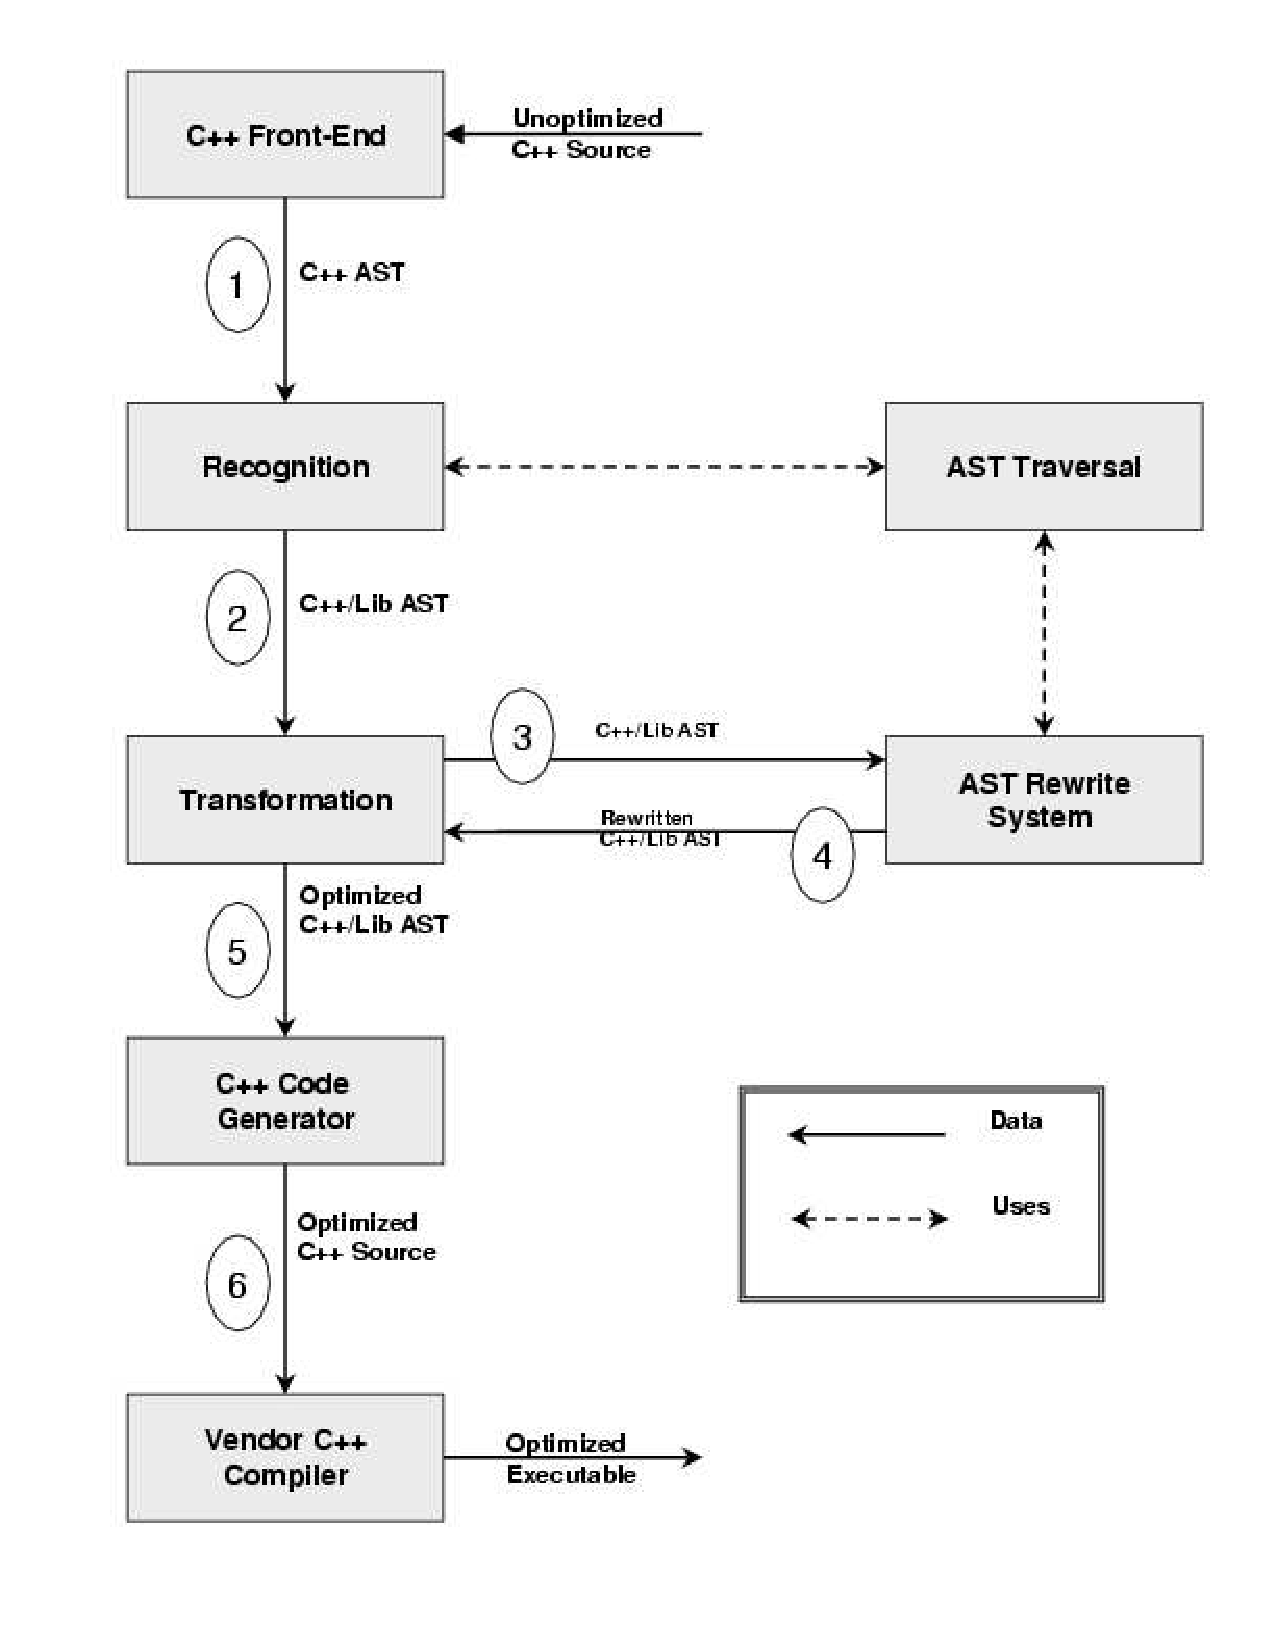
\includegraphics[height=1.0\linewidth,width=1.0\linewidth,angle=0]{rose-processing-phases}}
% the following line didn't work for me using acroread in Linux (tps 30Jun08) 
%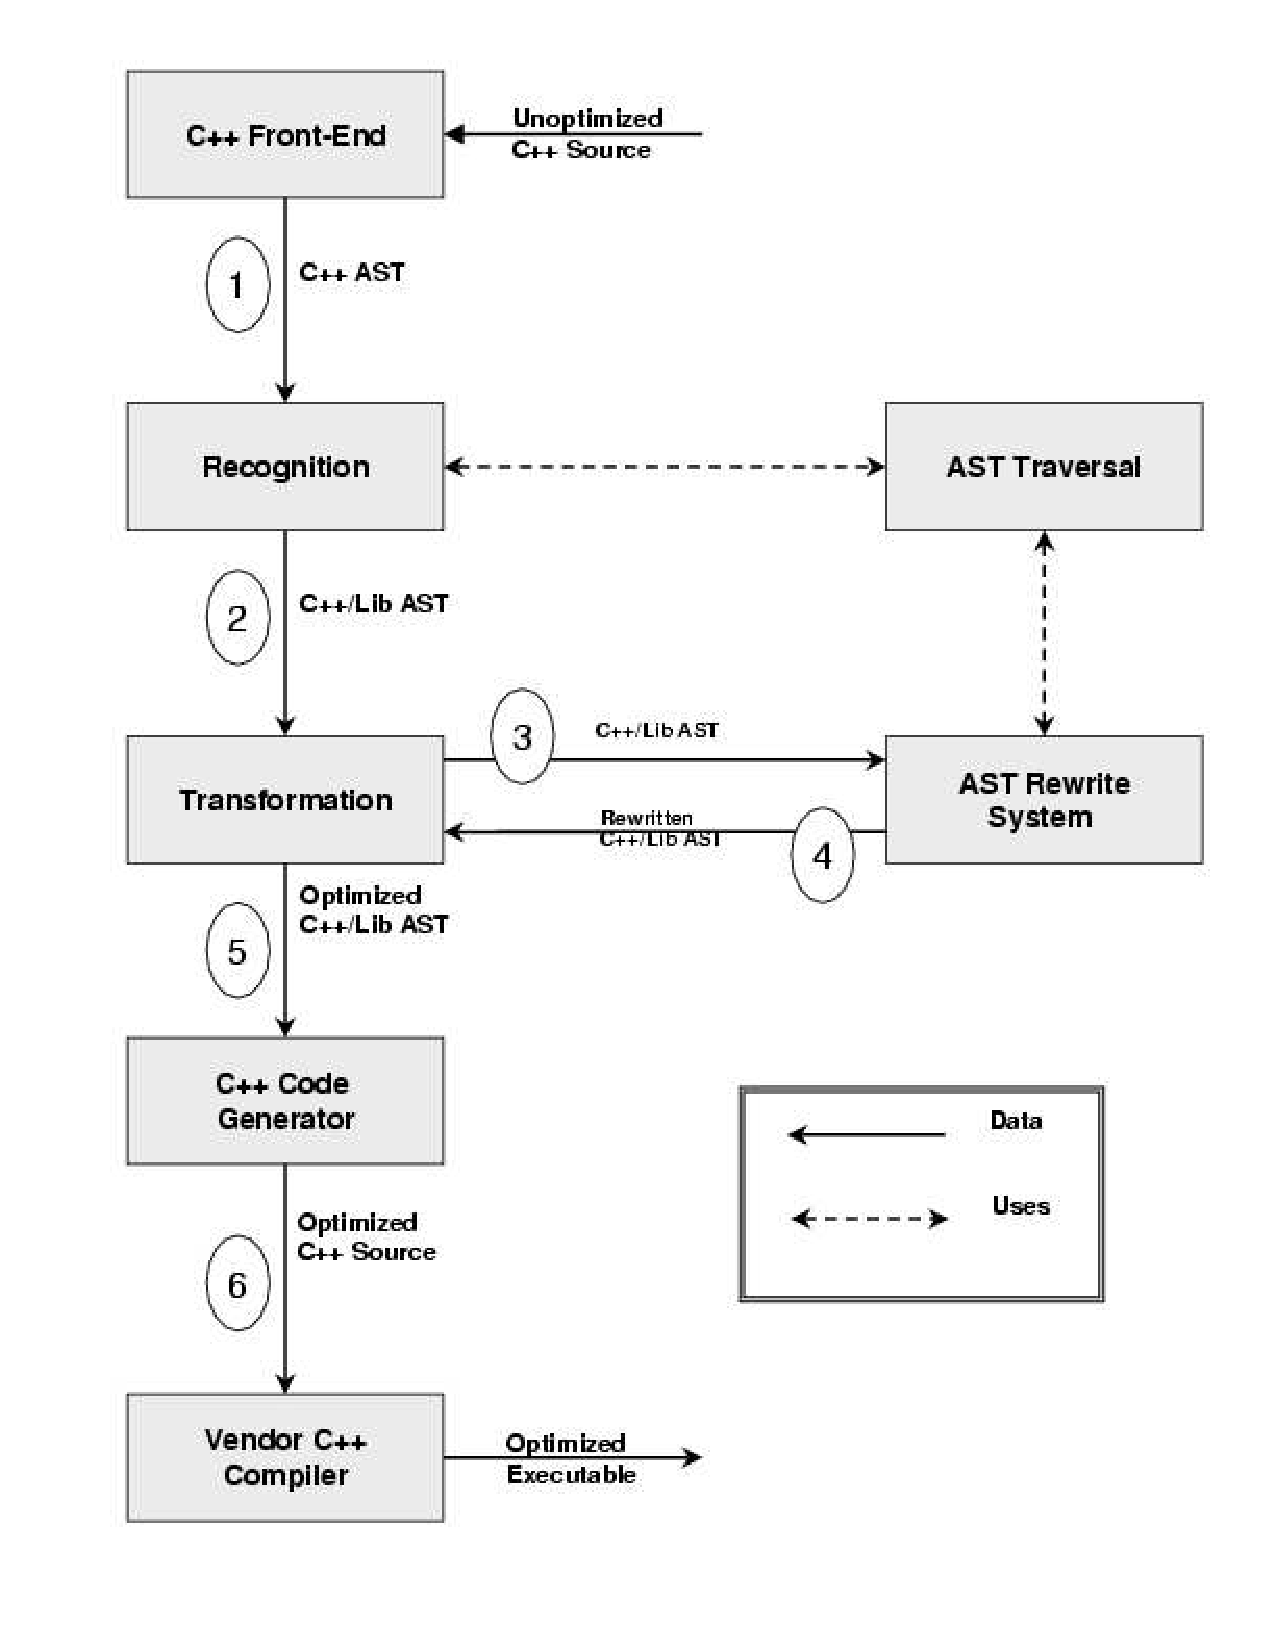
\includegraphics[trim=6.0in 0in 0in 0in,scale=0.5]{rose-processing-phases}
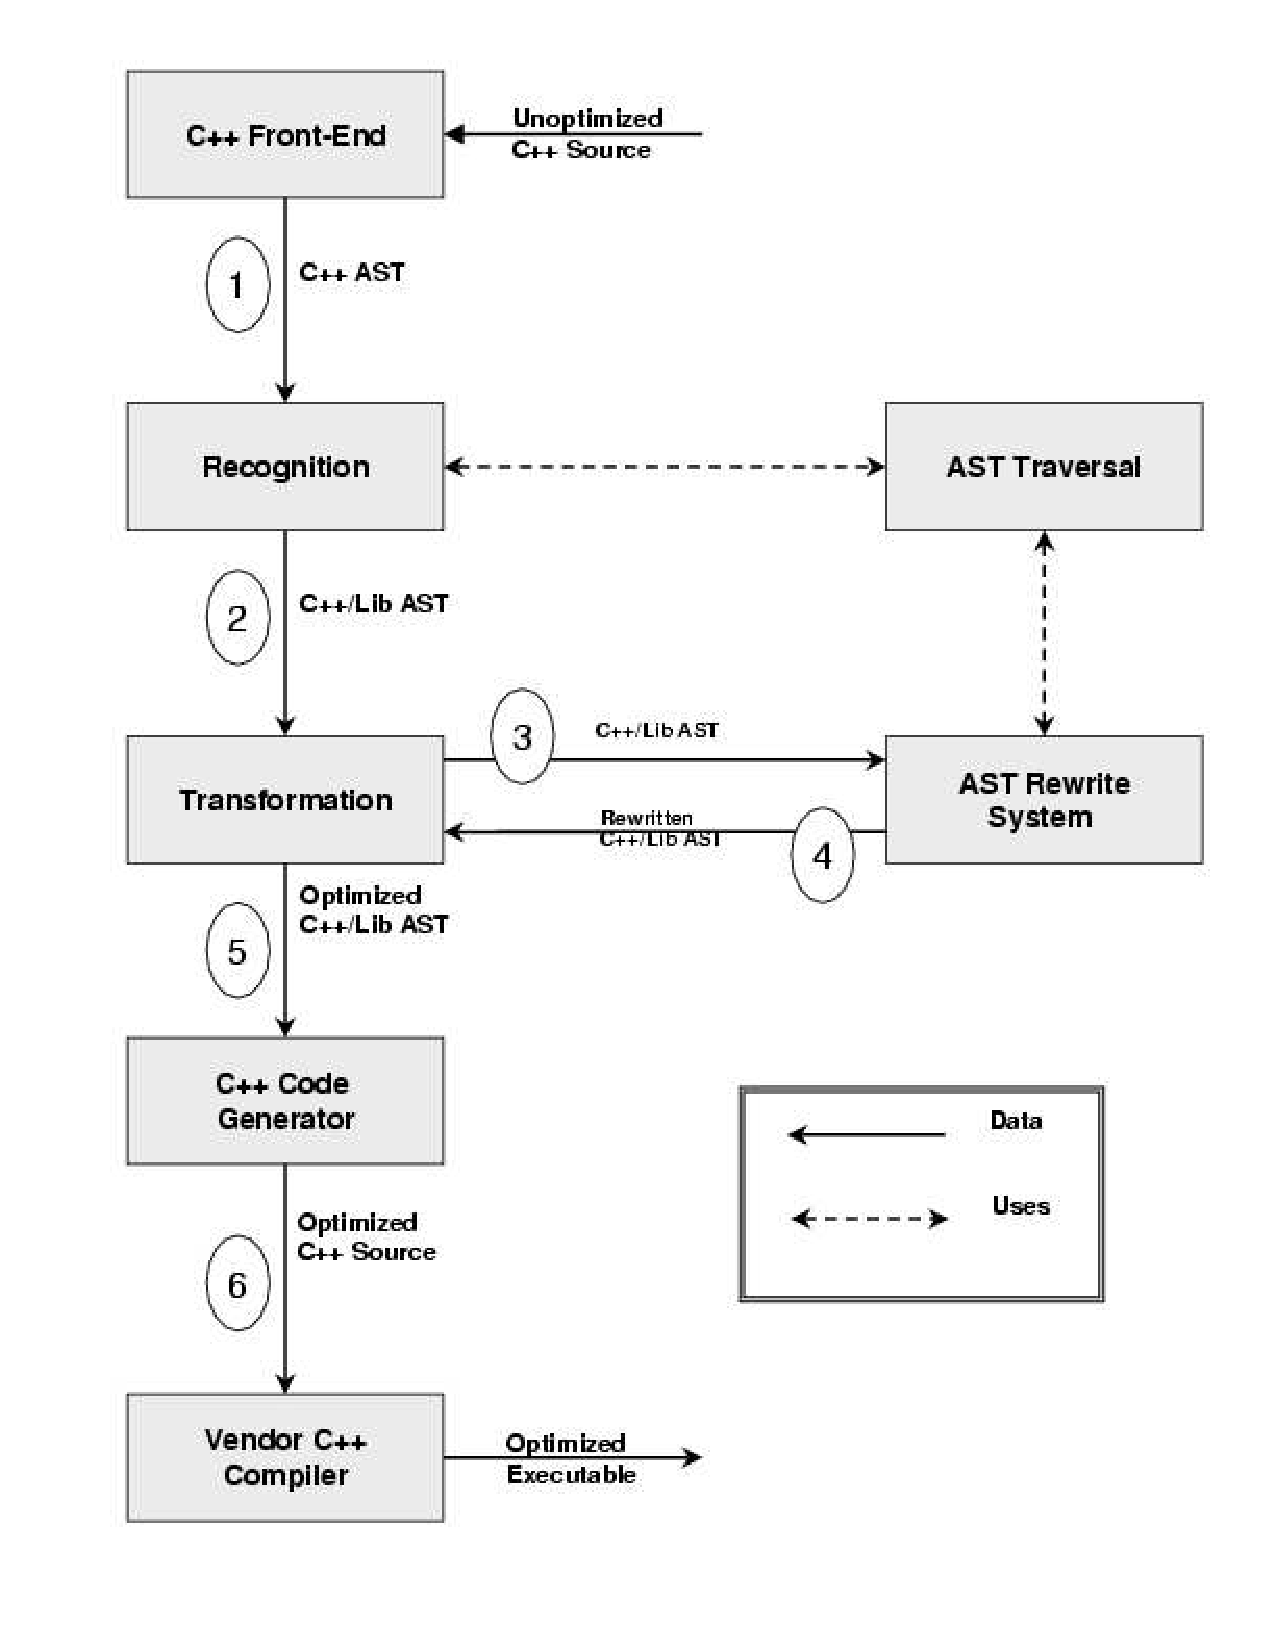
\includegraphics[scale=0.5]{rose-processing-phases}
\caption{Different phases of internal processing within translators built using ROSE infrastructure}
\label{introduction:phases}
\end{figure}



\section{ROSE Web Site}
    We have a ROSE Project Web page that can be accessed at the 
\htmladdnormallink{{\em ROSE}}{http://www.rosecompiler.org}
Web pages at
{\bf http://www.rosecompiler.org}.

This site is updated regularly with the latest documentation and software, as it is 
developed.
\footnote{All ROSE documentation is still in development}.


\section{ROSE Software/Documentation}
     ROSE is not yet released publicly on the Web, but is available
within the SciDAC Performance Evaluation Research Center (PERC) 
project and through limited collaborations with the developers
at universities and other laboratories.  Since the spring of 2006, we have made ROSE 
available via a password protected web page to all who have ask for access.
More information is available on the
\htmladdnormallink{ROSE}{http://www.rosecompiler.org} 
Web pages, located at:
{\bf http://www.rosecompiler.org}.
Web pages are updated regularly (postscript versions of 
documentation are available as well).

% When processing with latex2html use the -noinfo option to avoid generating
% a section ``About This Document'' which could be confused with this section.
\section{About This Manual}

   This section includes a description of what this manual
provides, how to use the manual, and the terminology related to
the examples.  
% Included in this introduction is 
An overview of the ROSE project is included. Error messages 
are contained in the Appendix (there are few at the moment).  
Further information is provided about
the ROSE Web site, where more information is available and where
the latest copy of the documentation is located.  This Web site will also be the
distribution site for ROSE, once it is made public; until then we welcome 
researchers to contact us directly to obtain pre-release versions of ROSE.

This manual is divided into several principal chapters.
Each chapter covers material that, in some cases, requires an understanding of
previous chapters. These are intended to simplify your use of this manual.
Each chapter is described briefly below:
\begin{itemize}
   \item {\bf Preface} \\
      This section briefly describes what this project is about.

   \item {\bf Acknowledgments} \\
      This section acknowledges contribution by many people over several years to the
      development of the ROSE project.

   \item {\bf Introduction} \\
      This chapter introduces why we have developed ROSE and some of its organization.

   \item {\bf Getting Started} \\
      This chapter walks the user through the configuration, compilation, installation,
      and testing of ROSE. Installation requirements are also explained. A small set of tests
      are available which verify the installation.

   \item {\bf Writing a Source-to-Source Translator} \\
      This chapter presents, by example, the details of writing a trivial translator using
      ROSE. 

   \item {\bf Overview of ROSE} \\
      This chapter presents details of specific features in ROSE.

   \item {\bf AST Query Library} \\
      This chapter presents work that has been completed to support simple and complex queries on the AST.

   \item {\bf AST Traversal} \\
      This chapter covers different ways to write AST traversals (operators on the
      AST). This chapter 
    % requires an understanding of the previous chapter, and 
      is required to understand the subsequent chapter on the AST Rewrite Mechanism.

   \item {\bf AST Rewrite Mechanism} \\ This chapter covers the details of how to use the 
      mechanism within ROSE for modifying the AST. This chapter describes how to write
      general transformations on the Abstract Syntax Tree (AST).   It builds on concepts
      from the previous chapter.

   \item {\bf Program Analysis} \\
      This chapter explains what program analysis is available within ROSE.

   \item {\bf Loop Transformations} \\
      This chapter explains the loop optimization work that has been done.

   \item {\bf SAGE III Intermediate Representation} \\
      This chapter details issues specific to the IR used in ROSE.

   \item {\bf Appendix} \\ This contains information that has not yet made its way
      into the manual.  Much of this information will later be integrated into the 
      User Manual, but until then, it is provided for reference.  This chapter will at some point 
      contain a reference to error messages (there are few at present, most abort upon
      error, just like a compiler).

   \item {\bf Developer's Appendix} \\
      This chapter contains information specific to development of ROSE, and thus mostly 
    of use only for ROSE developers.

   \item {\bf Frequently Ask Questions (FAQ)} \\
      This chapter contains a series of frequently ask questions (FAQ) about the ROSE project.

   \item {\bf Glossary} \\ 
      Terms and definitions that simplify the documentation are included in this section. 
      More will be added over time.

\end{itemize}

   A later version of the manual will include performance data on different machines
so that the use of different features in ROSE can be better understood.  This
work is incomplete at present (implemented, but not yet represented in the documentation).











\clearpage
%\newpage
\section{Preparation}
The preparation phase provides basic information about a target application's performance
characteristics. 
Such information can be obtained by many performance tools.
Currently, we accept performance data generated by both HPCToolkit and GNU gprof.
%Currently, the ROSE-HPCToolKit interface is used to accept performance data generated by HPCToolkit and GNU gprof.
%The interface is used to annotate ROSE AST with performance metrics to
%facilitate building automated performance analysis tools. 
%Detailed information about ROSE-HPCToolKit can be found in Chapter 44 of
%the ROSE tutorial. 
%We only give information relevant to autotuning below.

\subsection{Using HPCToolkit}
%The HPCToolkit~\cite{hpctoolkit} is developed at the Rice University to get
%performance metrics of the target application. 
The HPCToolkit~\cite{hpctoolkit}, developed at the Rice University, is an open source profile-based
performance analysis tool which samples the executions of optimized applications. 
No code
instrumentation is needed to use HPCToolkit. 
But debugging information (by compiling with
the -g option if GCC is used) in the binary executables is needed for the tool to
associate performance metrics with source language constructs.

After installation, a typical session of using HPCToolkit is given below:
{\mySmallFontSize
\begin{verbatim}
% Prepare the executable with debugging information
gcc -g smg2000.c -o smg2000 

% Sample one or more events for the execution, use wall clock here
hpcrun -e WALLCLK -- ./smg2000 -n 120 120 120 -d 3

% Convert the profiling result into a XML format
hpcproftt -p -D /home/liao6/svnrepos/benchmarks/smg2000 ./smg2000 \
  smg2000.WALLCLK.tux268.llnl.gov.10676.0x0 > result.xml

\end{verbatim}
}

\fixme{TODO: update the text when the latest release of HPCToolkit works
on 32-bit platforms}

%A SMG2000~\cite{BrownSemicoarsening2000} (Semicoarsening Multigrid Solver) benchmark from the ASCI Purple
%benchmark suite is chosen to exemplify the use of this system.

Fig.~\ref{fig:hpctoolkitSmg2000} shows the profiling results of SMG2000
using HPCToolkit. 
A statement in a loop takes more than 46\% execution time, which makes the
loop dominant, most expensive loop of the entire program.
\begin{figure}[htbp]  
	\centering
		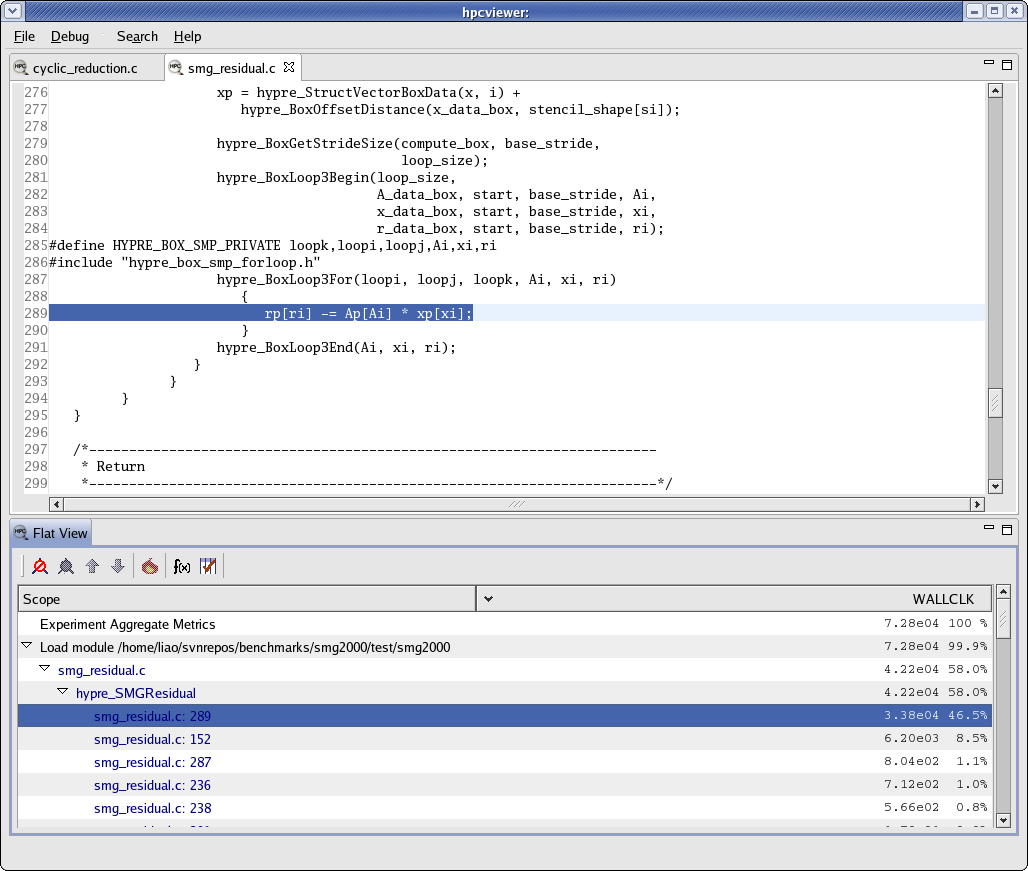
\includegraphics[width=0.9\textwidth]{hpctoolkit-smg2000.png}
	\caption{Profiling results of SMG2000 using HPCToolkit}
	\label{fig:hpctoolkitSmg2000}
\end{figure}

\subsection{Using gprof}
GNU gprof can generate line-by-line performance information for an
application. A typical session to generate such information is given below:
\begin{verbatim}
[liao@codes]$ gcc -g seq-pi.c -pg
[liao@codes]$ ./a.out
[liao@codes]$ gprof -l -L a.out gmon.out &>profile.result
\end{verbatim}

The option {\tt -l} tells gprof to output line-by-line profiling
information. 
{\tt -L} causes gprof to output full file path information, which is needed
for ROSE to accurately match performance data to source code.

An excerpt of an output file for smg2000 looks like the following:
{\scriptsize
\begin{verbatim}
Flat profile:

Each sample counts as 0.01 seconds.
  %   cumulative   self     
 time   seconds   seconds     name
 35.01     13.08    13.08     hypre_SMGResidual (/home/liao/smg2000/struct_ls/smg_residual.c:289 @ 804caa4)
  9.05     16.46     3.38     hypre_CyclicReduction (/home/liao/smg2000/struct_ls/cyclic_reduction.c:1130 @ 8054af4)
  8.40     19.60     3.14     hypre_SMGResidual (/home/liao/benchmarks/smg2000/struct_ls/smg_residual.c:291 @ 804cab9)
  7.67     22.46     2.87     hypre_CyclicReduction (/home/liao/smg2000/struct_ls/cyclic_reduction.c:910 @ 8053191)
  5.97     24.70     2.23     hypre_CyclicReduction (/home/liao/smg2000/struct_ls/cyclic_reduction.c:998 @ 8053a28)
  5.27     26.66     1.97     hypre_SMGResidual (/home/liao/smg2000/struct_ls/smg_residual.c:238 @ 804d129)
  2.86     27.73     1.07     hypre_SMGResidual (/home/liao/smg2000/struct_ls/smg_residual.c:287 @ 804cacb)
  2.28     28.59     0.85     hypre_CyclicReduction (/home/liaosmg2000/struct_ls/cyclic_reduction.c:853 @ 8052bae)
  2.07     29.36     0.78     hypre_CyclicReduction (/home/liao/smg2000/struct_ls/cyclic_reduction.c:1061 @ 8054450)
  1.79     30.03     0.67     hypre_SemiRestrict (/home/liao/smg2000/struct_ls/semi_restrict.c:262 @ 8056a8c)
  1.67     30.66     0.62     hypre_SemiInterp (/home/liao/smg2000/struct_ls/semi_interp.c:294 @ 8055d6c)
  1.12     31.07     0.42     hypre_CyclicReduction (/home/liao/smg2000/struct_ls/cyclic_reduction.c:1133 @ 8054b2f)
  0.96     31.43     0.36     hypre_CyclicReduction (/home/liao/smg2000/struct_ls/cyclic_reduction.c:912 @ 80531a6)
  0.87     31.76     0.33     hypre_StructAxpy (/home/liao/smg2000/struct_mv/struct_axpy.c:69 @ 806642c)
  0.80     32.06     0.30     hypre_CyclicReduction (/home/liao/smg2000/struct_ls/cyclic_reduction.c:1002 @ 8053a60)
  0.78     32.35     0.29     hypre_SMGResidual (/home/liao/smg2000/struct_ls/smg_residual.c:236 @ 804d14b)
  0.72     32.62     0.27     hypre_CyclicReduction (/home/liao/smg2000/struct_ls/cyclic_reduction.c:1063 @ 8054462)
  0.60     32.84     0.23     hypre_SMGAxpy (/home/liao/smg2000/struct_ls/smg_axpy.c:69 @ 8064970)
  0.59     33.06     0.22     hypre_CycRedSetupCoarseOp (/home/liao/smg2000/struct_ls/cyclic_reduction.c:369 @ 8051149)
  0.59     33.28     0.22     hypre_SMGResidual (/home/liao/smg2000/struct_ls/smg_residual.c:240 @ 804d146)
  0.51     33.48     0.19     hypre_StructVectorSetConstantValues (/home/liao/smg2000/struct_mv/struct_vector.c:578 @ 806fedc)
  0.48     33.66     0.18     hypre_SMGSetupInterpOp (/home/liao/smg2000/struct_ls/smg_setup_interp.c:292 @ 804ea04)
  0.46     33.83     0.17     hypre_SemiInterp (/home/liao/smg2000/struct_ls/semi_interp.c:227 @ 80556e8)
  0.40     33.98     0.15     hypre_CyclicReduction (/home/liao/smg2000/struct_ls/cyclic_reduction.c:855 @ 8052bd4)
  0.40     34.12     0.15     hypre_StructMatrixInitializeData (/home/liao/smg2000/struct_mv/struct_matrix.c:359 @ 80678b0)
  ...
\end{verbatim}
}



%We use the self seconds associated with each source line and attach them to
%ROSE AST as AST attributes named WALLCLK.


\clearpage
\section{Code Triage and Transformations}
The second phase (shown in Fig.~\ref{fig:phase12}) includes code triage and a set of code transformations. 
Code triage relies on a ROSE-based tool interface to read in both source files and performance information of
the input application.
It then conducts various automated or user-directed analyses to identify
problematic code segments, such as loops. 
Finally, the identified code segments are extracted (also called outlined) into separated routines so they can be individually
optimized by empirical methods. 
%Since the analysis is on the AST or other graphs built
%using ROSE and uses the performance data stored as attributes, these analyses are
%expressed using traversals in ROSE.
\begin{figure}[htbp]
\vspace{5ex}
       \centering
               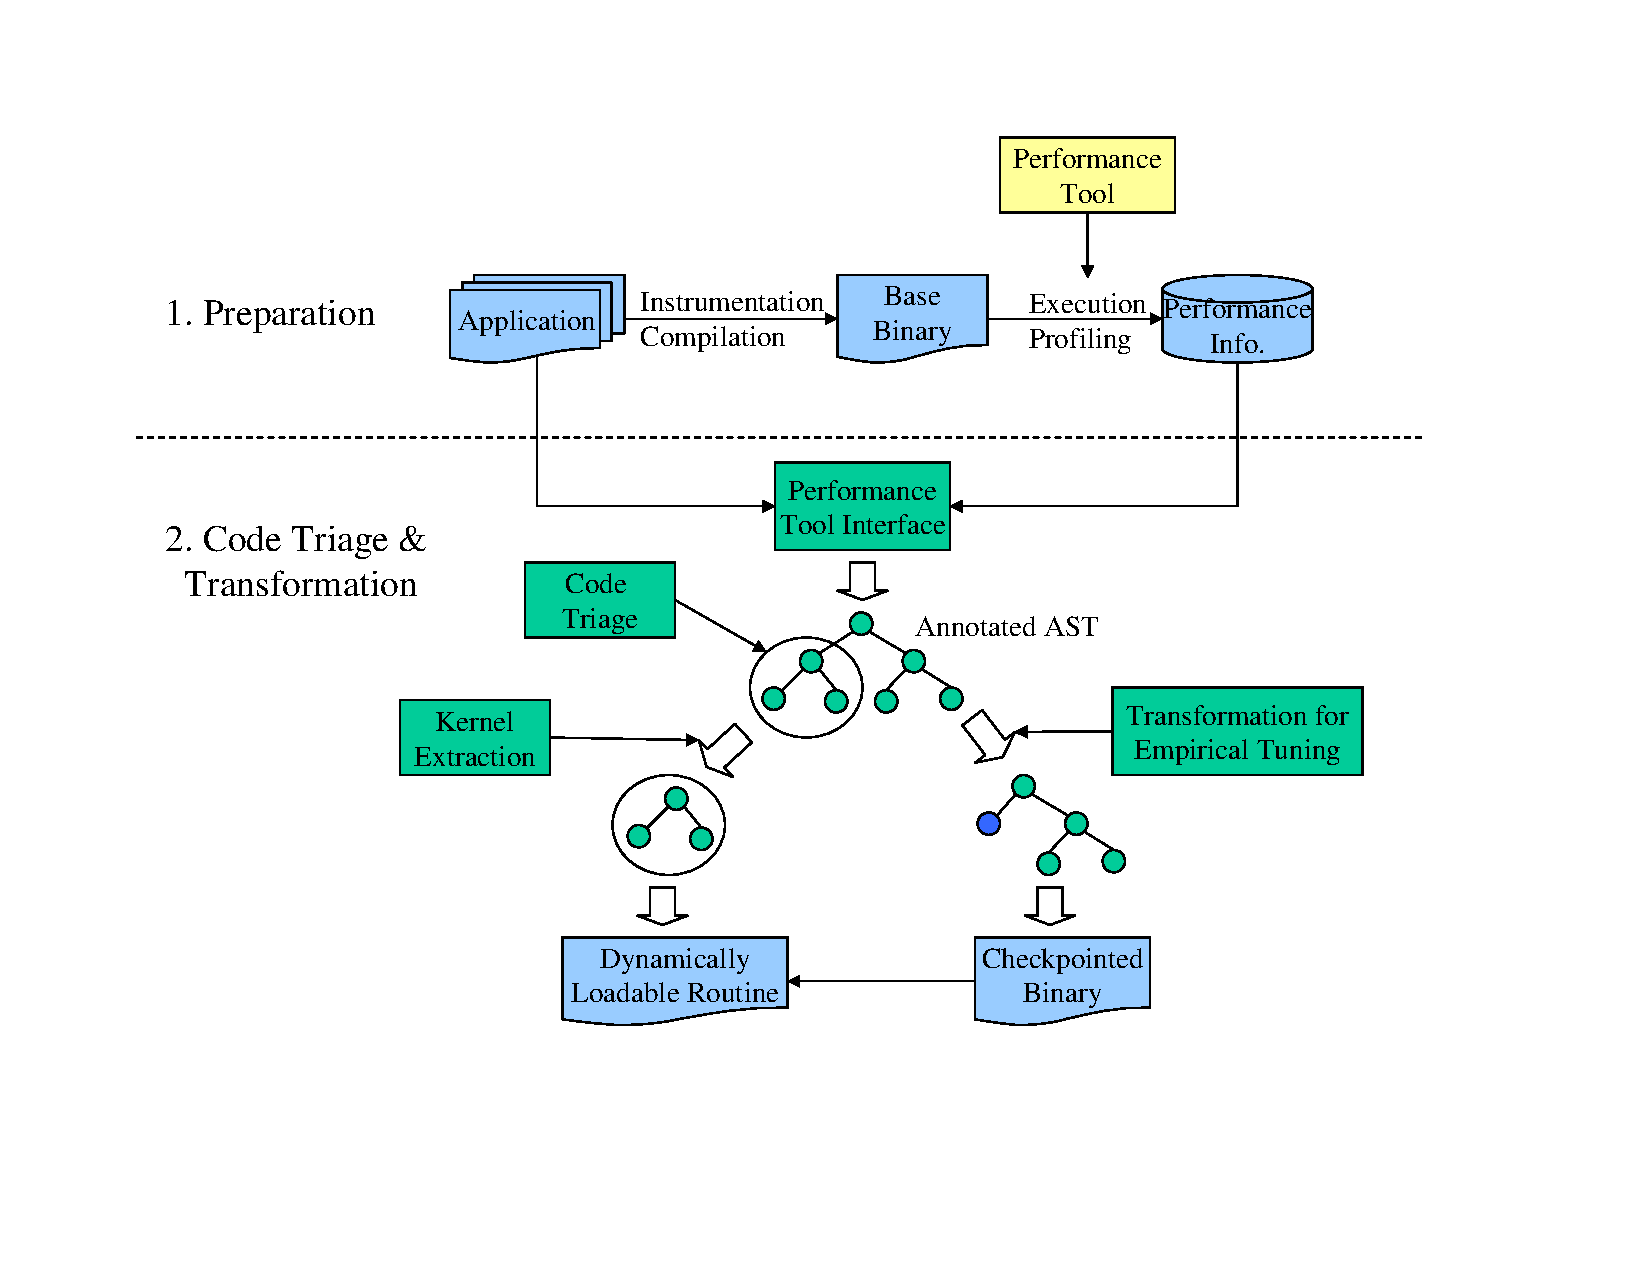
\includegraphics[width=1.2\textwidth]{phase12.pdf}
       \caption{Phase 1 and 2 of the autotuning system}
       \label{fig:phase12}
\end{figure}

%---------------------------------------------------
\subsection{Invoking Code Triage}
The source code for code triage is located in
\textit{rose/projects/autoTuning/autoTuning.C}. 
It already has initial implementation to call ROSE's tool interface,
conduct simple code triage, and finally extract kernels using ROSE's AST
outliner. 

With the input application and its performance result available, 
%a straightforward method is used to identify the most time-consuming
%statements in the code.  
%Loop nests containing those statements are reported as a
%tuning candidate, if the loop nests exist.
users can invoke the ROSE-based code triage by using the following command:

{\mySmallFontSize
\begin{verbatim}
autoTuning -c  jacobi.c -rose:hpct:prof jacobi-raw.xml \
-rose:autotuning:triage_threshold 0.8 -rose:outline:output_path "tests"
\end{verbatim}
}

The command above provides an input source file and its corresponding XML-format performance data generated by HPCToolkit.
It asks the code triage program to find the most time-consuming 
loops which account for just above 80\% of the total execution time. 
The identified loops will be automatically extracted to separated,
source files and saved into an output path named \textit{tests}.

Users can also enable code triage only without calling outlining. 
The performance data can come from GNU gprof. 
An example is given below:

%{\scriptsize
{\mySmallFontSize
\begin{verbatim}
# example command line to perform code triage only.
autoTuning  -c jacobi.c -rose:autotuning:triage_only -rose:gprof:linebyline jacobi.gprof.txt 

# the output is a list of abstract handles and 
# their corresponding execution time percentage
-----------------------------------------------------------------
The abstract handles for hot statements exceeding the threshold are:
Project<numbering,1>::SourceFile<name,/home/liao6/jacobi.c>::\
ExprStatement<position,193.9-194.76>
0.382
Project<numbering,1>::SourceFile<name,/home/liao6/jacobi.c>::\
ExprStatement<position,196.9-196.45>
0.3643
Project<numbering,1>::SourceFile<name,/home/liao6/jacobi.c>::\
ExprStatement<position,188.9-188.29>
0.11
-----------------------------------------------------------------
The abstract handles for enclosing loops for hot statements exceeding the
threshold are:
Project<numbering,1>::SourceFile<name,/home/liao6/jacobi.c>::\
ForStatement<position,190.5-198.7>
0.8189
\end{verbatim}
}

The above example command identifies a list of the most time-consuming statements and loops and reports them using abstract handles. 
The report will end once the sum of execution time of the statements or
loops reach or exceed a preset threshold (default is 75\% of the total execution time). 

We explain some details for the implementation of code triage and
autotuning-related transformations in the following subsections.
%----------------------------------------
\subsection{Tool Interface}
%A ROSE tool interface is required for understanding the performance results of each
%external performance tool. 
ROSE has a performance tool interface, called ROSE-HPCT,
in its distribution to accept performance results generated by external
performance tools .  
%Please follow the instructions from ROSE
%Tutorial's Chapter ROSE-HPCToolkit Interface to enable and use this module. 
Basically, it reads in the XML files generated from HPCToolkit and attaches performance metrics to
the ROSE AST representing the corresponding source code.
It can handle macro expansions during the metric match process.
When necessary, all performance metrics are also propagated from statement
levels to loop, function, and file levels. 
Similarly, it also accepts the line-by-line performance data generated by GNU
gprof.
%Currently, the ROSE-HPCToolKit interface is used to accept performance
%data generated by HPCToolkit and GNU gprof.
%The interface is used to annotate ROSE AST with performance metrics to
%facilitate building automated performance analysis tools. 
Detailed information about ROSE-HPCToolKit can be found in Chapter 44 of
the \htmladdnormallink{ROSE Tutorial}{http://www.rosecompiler.org/ROSE_Tutorial/ROSE-Tutorial.pdf}.
%We only give information relevant to autotuning below.

The code triage program uses the following code to invoke ROSE-HPCT.

{\mySmallFontSize
\begin{verbatim}
int main(int argc, char * argv[]) 
{
  vector<string> argvList (argv, argv+argc);
  // Read into the XML files
  RoseHPCT::ProgramTreeList_t profiles = RoseHPCT::loadHPCTProfiles (argvList);
  // Create the AST tree
  SgProject * project = frontend(argvList);
  //Attach metrics to AST , last parameter is for verbose
  RoseHPCT::attachMetrics(profiles, project,project->get_verbose()>0);
  //...
}
\end{verbatim}
}

%%----------------------------------------
%\subsection{Code Triage}
%A code triage module examines the AST annotated with
%performance metrics to locate problematic code portions (we call these code portions
%as autotuning targets).
%Currently, a straightforward top-down method is used to identify a hot spot
%in the code from the most time consuming file and then the loop nests containing such spot is reported as a
%tuning candidate, if the loop nests exist. The example code is shown below:
%\fixme{ROSE's AST merge could be used in the future to have a global view
%of AST merged from multiple source files.}
%
%{\mySmallFontSize
%\begin{verbatim}
% std::string hot_file = findHottestFile(fileMetrics);
% SgNode* hot_node=findHottestStatement(file, nodesWithMetrics);
% SgForStatement* target_loop= findTargetLoop(hot_node);
%
%\end{verbatim}
%}
%
%Code triage is also designed to suggest a set of potentially beneficial optimizations and
%their configuration ranges to improve the performance.
%\fixme{TODO need to implement this by compiler analysis. We manually 
% use the limited optimization choices, such as loop unrolling, by default for now.}
%
% DQ: Liao, what is the best entry point for me to write such a module/traversal.
% I think it would be good to have this in place before we release this document.
% I will be happy to write this part.

%----------------------------------------
\subsection{Kernel Extraction: Outlining}
Each of the identified tuning targets, often loops, will be extracted from the original code to
form separated functions (or routines). 
The ROSE AST outliner is invoked to generate such functions. 
%It replaces a block of consecutive statements with a function call to a newly generated
%function containing those statements. 
This kernel extraction step can be automatically invoked by the code triage
program or manually initiated by users via the outliner's command line
interface. 

The ROSE AST outliner handles multiple input languages, including C, C++ and
recently Fortran.  It also provides both command line and programming interfaces for users
to specify the targets to be outlined.  
Detailed information of using the ROSE outliner can be found in
Chapter 27 of the \htmladdnormallink{ROSE
Tutorial}{http://www.rosecompiler.org/ROSE_Tutorial/ROSE-Tutorial.pdf}.
You can also refer to a paper~\cite{LiaoEffective2009} for the algorithm we use to outline kernels. 
%More details of the ROSE AST outliner are
%available in the ROSE Tutorial's Chapter, Function Outlining using the AST Outliner.
For the code triage program, the programming interface of the Outliner is
used as below:

{\mySmallFontSize
\begin{verbatim}
  // recognize options for outliner
  Outliner::commandLineProcessing(argvList);
  ...
 SgForStatement* target_loop= findTargetLoop(hot_node);
 if (isOutlineable (target_loop))  
   outline(target_loop);
\end{verbatim}
}

The ROSE AST outliner accepts user options to further guide its internal
behavior. \lstinline{-rose:outline:parameter_wrapper } will wrap all
parameters of the outlined function into an array of pointers. 
\lstinline{-rose:outline:new_file} will separate the outlined function into
a new source file to facilitate external tools for further handling.
\lstinline{-rose:outline:use_dlopen} will transform the code to use
\lstinline{dlopen()} and \lstinline{dlsym()} to dynamically load the
outlined function from a library.

For the SMG2000 example, the most time-consuming loop is outlined and a call to it is used
to replace the loop in the original code. 
The loop is actually expanded from a macro
\lstinline{hypre_BoxLoop3For()}. 
ROSE is able to identify it after a bottom
up metrics propagation phase in ROSE-HPCT. 
%\fixme{Need to come up a way to automatically handle this, Should we
%do it within the outliner itself or before calling the outliner?})
The kernel extraction's result is shown in the following code listing:
\lstset{language={C},basicstyle=\scriptsize} 
\lstinputlisting{smg2000_outlined.fold.c}
\lstset{language={C},basicstyle=\small} 

%\fixme{TODO 
%   Also we should evaluate the overhead of this
%   step if the final result is an optimized function represented as a separate 
%   file (potentially disables some optimizations).  In the final assembly 
%   we could remove the dynamic linking, but the Makefile would have to be modified which
%   gets messy for an automated system.}

The ROSE outliner uses a variable cloning method to
avoid using pointer dereferencing within the outlined computation kernels. 
The method is based on usage of a variable that is passed by reference and
accessed
via pointer-dereferencing by classic outlining algorithms.
Such a variable is used either by value or by address within an outlining
target.
For the C language, using the variable by address occurs when the
address operator
is used with the variable (e.g. \lstinline{&X}).
C++ introduces one more way of using the variable by address:
associating the variable with a reference type
(\lstinline{TYPE & Y = X;} or using the variable as an argument for a
 function's parameter of a reference type).
If the variable is not used by its address,
a temporary clone variable of the same type (using \lstinline{TYPE clone;})
can be introduced to substitute its uses within the outlined function.
The value of a clone has to be
initialized properly (using \lstinline{clone = * parameter;})
before the clone participates in computation.
After the computation, the original variable must be set to the clone's
final value
(using \lstinline{*parameter = clone}).
By doing this, many pointer dereferences introduced by the classic
algorithm can be avoided.
\fixme{We are working on using liveness analysis to further eliminate unnecessary
value assignments.}

For easier interaction with other tools, the outlined function is separated
into a new source file, usually named after 
the function name.  
The ROSE outliner will recursively find and copy all dependent type declarations
into the new file to make it compilable.
For the SMG2000 example, a file named out\_1\_6755\_\_.orig.c 
is generated and it only contains the function body of \lstinline{OUT_1_6755__()}. 
This file will be transformed by a parameterized optimizer to a kernel
variant named OUT\_\_1\_\_6755\_\_.c and further compiled into a dynamically
loadable routine.

A sample makefile to generate the .so file is given below: 

{\mySmallFontSize
\begin{verbatim}
[liao@localhost smg2000] cat makefile-lib
lib:OUT__1__6755__.so
OUT__1__6755__.o:OUT__1__6755__.c
        gcc -c -fpic OUT__1__6755__.c
OUT__1__6755__.so:OUT__1__6755__.o
        gcc -shared -lc -o OUT__1__6755__.so OUT__1__6755__.o
clean:
        rm -rf OUT__1__6755__.so OUT__1__6755__.o
\end{verbatim}
}

%----------------------------------------
\subsection{Transformations for Autotuning}
The call site of the outlined function in the source code has to be further transformed to support empirical optimization. 
These transformations include:
\begin{itemize}
\item using \lstinline{dlopen()} to open a specified .so file containing
the outlined target and calling the function found in the file,
\item adding performance measuring code to time the call of the outlined target function.
\item transforming code to support checkpointing the execution right before
\lstinline{dlopen()} opening the library source file so multiple variants of the file can be used to test optimization choices empirically when the program is restarted multiple times.
\end{itemize}
%\fixme{TODO the code translations in this sub section are manually done
%now. We will start to
%implement them once the translation methods are agreed on by partners.}
%----------------------------------------
\subsubsection{Calling a Function Found in a .so File}
As mentioned earlier, the outlined function containing the target kernel is
stored in a separated source file, which will be transformed into a kernel variant
and then compiled to a dynamically loadable library. 
The original source code has to be transformed to open the library file,
find the outlined function, and finally call it using the right
parameters. An example of the resulting transformation on the function containing the
outlined loop is given below:
\lstset{language={C}, basicstyle=\scriptsize}
\lstinputlisting{smg2000_dlopen.c}

\subsubsection{Timing the Call}
The call to the outlining target kernel should be timed to get the
evaluation results during the empirical optimization. 
We instrument the call as follows to get the performance evaluation of a
kernel variant. 
More accurate and less intrusive methods based on hardware
counters can also be used in the future. 

{\mySmallFontSize
\begin{verbatim}
//save timing information into a temporary file

remove("/tmp/peri.result");
time1=time_stamp();
// parameter wrapping statements are omitted here
(*OUT__1__6755__)(__out_argv1__1527__);

time2=time_stamp();
FILE* pfile;
pfile=fopen("/tmp/peri.result","a+");
if (pfile != NULL)
{
  fprintf(pfile,"%f\n",time2-time1);
  fclose(pfile);
}
else
  printf("Fatal error: Cannot open /tmp/peri.result!\n");

\end{verbatim}
}

%----------------------------------------
\subsubsection{Checkpointing and Restarting}
In order to efficiently evaluate hundreds or even thousands of kernel
variants, we use a checkpointing and restarting method to measure the time
spent on calling the kernel without unnecessarily repeating the execution
before and after calling the kernel.  This allows the full context (state) 
of the application to be used in the evaluation of the kernel performance.
\fixme{need to discuss the drawbacks, e.g. missing cache warmup; and how that
might be addressed in the future by pushing back the checkpoint start and 
transformations to the checkpointed program (later).}

The Berkeley Lab Checkpoint/Restart (BLCR) library~\cite{blcrWeb} was selected for its
programmability, portability and robustness. 
BLCR is designed to support asynchronous checkpointing, which means a running process
is notified by another process to be checkpointed first, but the exact checkpointing
action happens on an indeterministic point later on. 
This default behavior is not desired for our purpose since we want an
accurate source position to do the checkpointing. 
Fortunately, BLCR's library does provide some internal functions to help
us initiate synchronous (immediate) checkpointing, though not well documented. 
After some trial and error rounds, we use the following code transformation
to have a synchronous checkpointing using the blcr-0.8.2 release.
The idea is to have a running program to notify itself to initiate a checkpointing. 
The program is then blocked until the request is served. 

To support BLCR, we have transformed the original source code in two locations.
% Two places in the source files have to be changed. 
The first location is the file where the main() function exists. We add the necessary
header files and initialization codes for using BLCR.  For example:
\lstset{language={C}, basicstyle=\scriptsize}
\lstinputlisting{smg2000_checkpoint.c}
% \lstset{language={C}, basicstyle=\small}

The second place is the actual source line to initiate the checkpointing. 
A checkpoint argument structure is filled out first to customize the
behavior we want, including the scope, target, memory dump file,
consequence, and so on. A blocking phase is put right after
\lstinline{cr_request_checkpoint()} to have an immediate checkpointing.
Our goal is to stop the executable right before opening the .so file so
a different kernel variant can be compiled into the .so file each time. 
The execution will be restarted multiple times so multiple variants can 
be evaluated this way. 

\lstset{language={C}, basicstyle=\scriptsize}
\lstinputlisting{smg2000_checkpoint2.c}
% \lstset{language={C}, basicstyle=\small}

Only these minimum transformations are needed to build the target application to support
BLCR. We choose the static linking method to support BLCR as follows.
The BLCR library is linked with the final executable. 

{\mySmallFontSize
\begin{verbatim}
smg2000: smg2000.o
        @echo  "Linking" \$@ "... "
        \${CC} -o smg2000 smg2000.o \${LFLAGS} -lcr
\end{verbatim}
}

The checkpointed binary has to be executed once to generate a memory dump
file (process image), which can then be reused multiple times to restart the execution 
immediately before the line where \lstinline{dlopen()} is invoked to evaluate multiple
variants of the optimization target kernel.

{\mySmallFontSize
\begin{verbatim}
[liao@localhost test] ./smg2000 -n 120 120 120 -d 3
current process ID is 6028
Running with these driver parameters:
  (nx, ny, nz)    = (120, 120, 120)
  (Px, Py, Pz)    = (1, 1, 1)
  (bx, by, bz)    = (1, 1, 1)
  (cx, cy, cz)    = (1.000000, 1.000000, 1.000000)
  (n_pre, n_post) = (1, 1)
  dim             = 3
  solver ID       = 0
=============================================
Struct Interface:
=============================================
Struct Interface:
  wall clock time = 0.550000 seconds
  cpu clock time  = 0.540000 seconds
Checkpoiting: stopping here ..
Killed
\end{verbatim}
}

A context dump file named dump.yy will be generated by BLCR as the
checkpointing result. This dump file will be used to restart the execution using
the command: \lstinline{cr_restart dump.yy}.

\section{Empirical Tuning}
The actual empirical tuning (shown in Fig.~\ref{fig:phase3}) is conducted via the cooperation of several
components: a search engine, a parameterized transformation tool, and 
the previously introduced checkpointing/restarting library.
The basic idea is that:
1) a set of pre-selected transformations and their corresponding configuration
   ranges are given (by the code triage module) and converted into an integral
   search space; 
2) the search engine evaluates points from the search space by driving the parameterized
   transformation tool to generate kernel variants and restarting the checkpointed binary
   to run the variants one by one.
\begin{figure}[htbp]
       \centering
               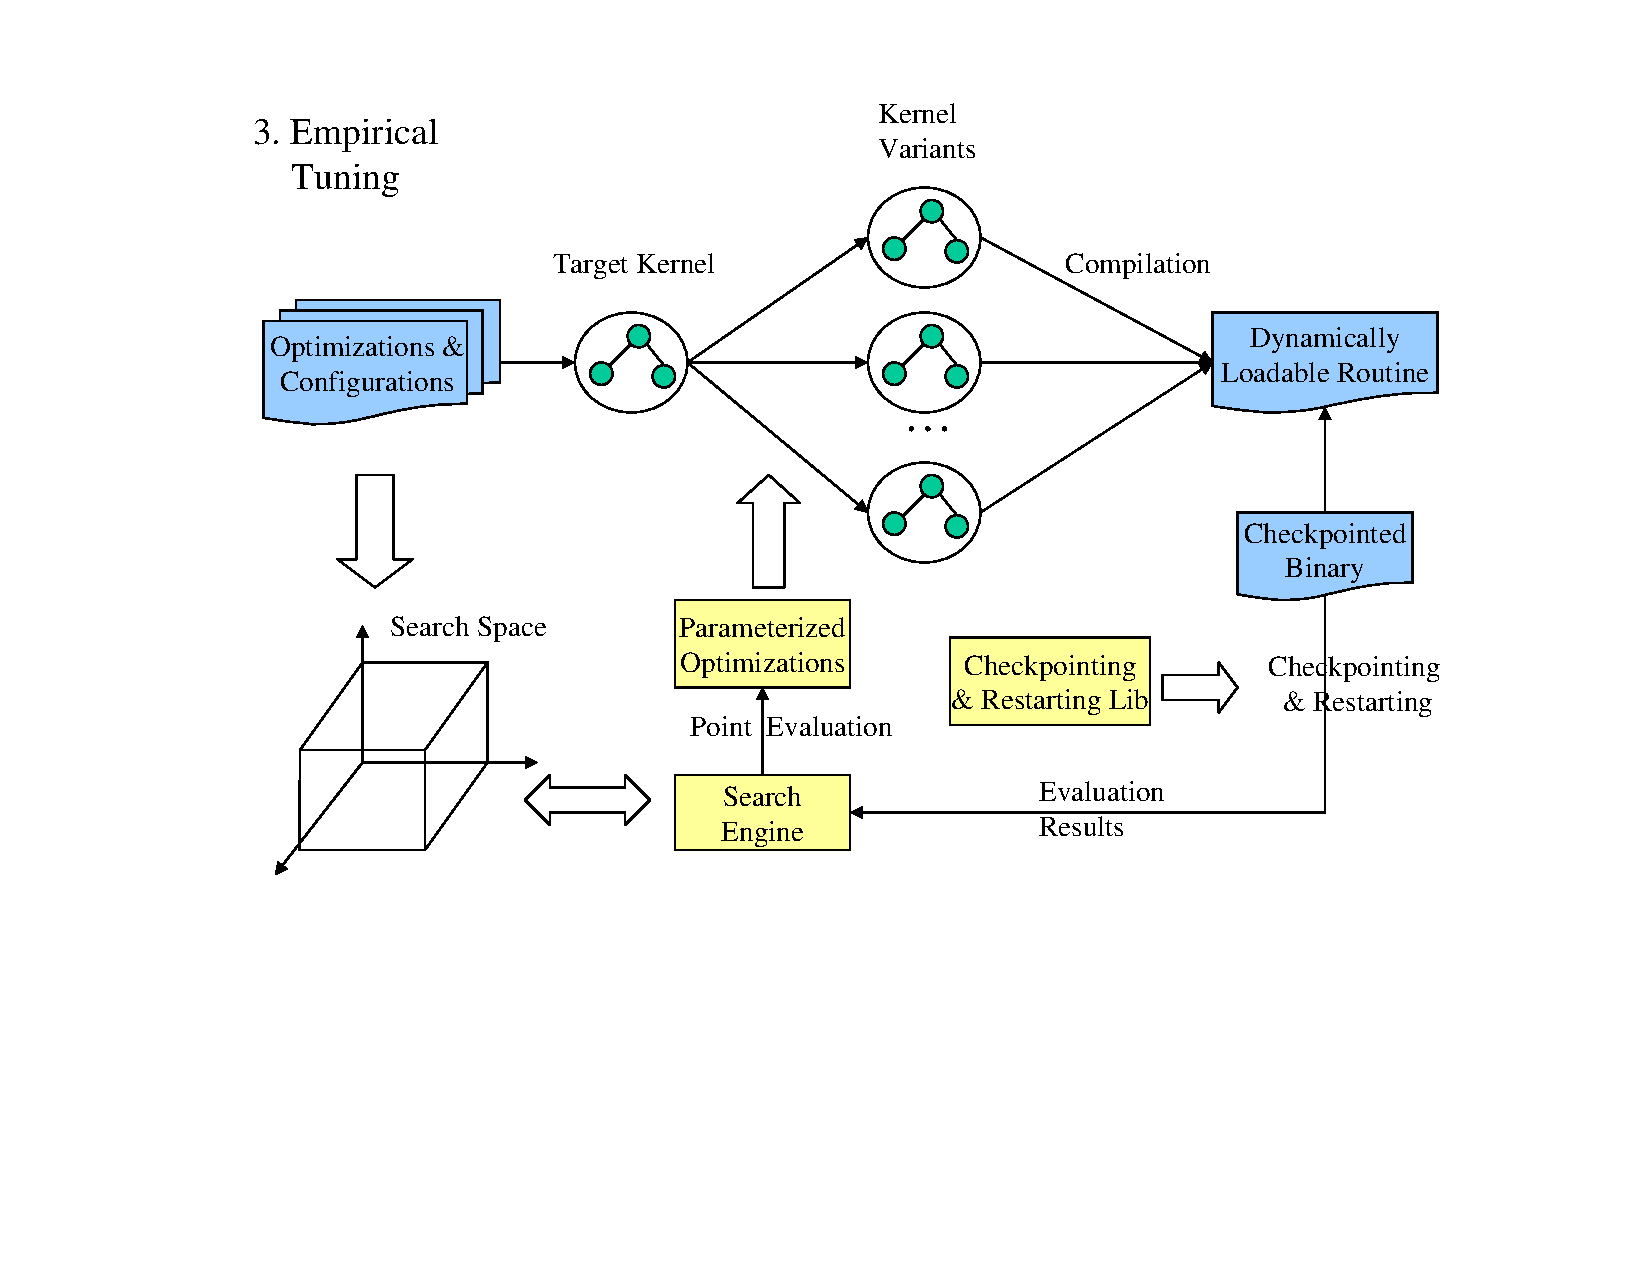
\includegraphics[width=1.2\textwidth]{phase3.pdf}
       \caption{Phase 3 of the autotuning system}
       \label{fig:phase3}
\end{figure}

%--------------------------------------------------
\subsection{Parameterized Transformation Tools}
Several choices exist to generate kernel variants, they include
POET~\cite{YiPOET2007},
CHiLL~\cite{ChenCHiLL2008}, and the ROSE loop translators. We take POET as an example here. 

POET (Parameterized Optimizations for Empirical
Tuning) developed by Dr.~Qing~Yi under contract with University of
Texas at San Antonio (UTSA), is an efficient language and tool to express hundreds or
thousands of complex code transformations and their configurations using a small set
of parameters.  It is especially relevant to the evaluation of large-scale search spaces
as part of empirical tuning and is orthogonal to any specific search strategy.

Using command line options and a configuration file, users can direct POET to apply a set
of specified transformations with desired configurations on selected code portions. 
Also, the target kernel has to be instrumented to aid POET in the process. 
Detailed POET user instructions can be found at its official website~\cite{poetWeb}.
For example, the SMG2000 kernel has the following format to support
POET:
\begin{figure}[!ht]
\centering
\lstset{language=C, basicstyle=\scriptsize}
\begin{lstlisting}
void
OUT__1__6755__ (void **__out_argv)
{
  int Ai =  *((int *)(__out_argv[20]));
  int xi =  *((int *)(__out_argv[19]));
  int ri =  *((int *)(__out_argv[18]));
  double *Ap =  *((double **)(__out_argv[17]));
  double *xp =  *((double **)(__out_argv[16]));
  double *rp =  *((double **)(__out_argv[15]));
  int loopi =  *((int *)(__out_argv[14]));
  int loopj =  *((int *)(__out_argv[13]));
  int loopk =  *((int *)(__out_argv[12]));
  int hypre__sx1 =  *((int *)(__out_argv[11]));
  int hypre__sy1 =  *((int *)(__out_argv[10]));
  int hypre__sz1 =  *((int *)(__out_argv[9]));
  int hypre__sx2 =  *((int *)(__out_argv[8]));
  int hypre__sy2 =  *((int *)(__out_argv[7]));
  int hypre__sz2 =  *((int *)(__out_argv[6]));
  int hypre__sx3 =  *((int *)(__out_argv[5]));
  int hypre__sy3 =  *((int *)(__out_argv[4]));
  int hypre__sz3 =  *((int *)(__out_argv[3]));
  int hypre__nx =  *((int *)(__out_argv[2]));
  int hypre__ny =  *((int *)(__out_argv[1]));
  int hypre__nz =  *((int *)(__out_argv[0]));
  for (loopk = 0; loopk < hypre__nz; loopk+=1) 
  {
    for (loopj = 0; loopj < hypre__ny; loopj+=1) 
    {
      for (loopi = 0; loopi < hypre__nx; loopi+=1)  //@BEGIN(nestI)
      {
        {
          rp[ri] -= ((Ap[Ai]) * (xp[xi]));
        }
        Ai += hypre__sx1;
        xi += hypre__sx2;
        ri += hypre__sx3;
      }
      Ai += (hypre__sy1 - (hypre__nx * hypre__sx1));
      xi += (hypre__sy2 - (hypre__nx * hypre__sx2));
      ri += (hypre__sy3 - (hypre__nx * hypre__sx3));
    }                                             //@END(nestI:Nest)
    Ai += (hypre__sz1 - (hypre__ny * hypre__sy1));
    xi += (hypre__sz2 - (hypre__ny * hypre__sy2));
    ri += (hypre__sz3 - (hypre__ny * hypre__sy3));
  }
 // some code omitted here...
}
\end{lstlisting}
  \caption{the SMG 2000 kernel}
    \label{Fig:smg2000kernel}
\end{figure}
%  for (loopk = 0; loopk < *hypre__nz; loopk+=1)
%    {
%      for (loopj = 0; loopj < *hypre__ny; loopj+=1)
%        {
%          for (loopi = 0; loopi < *hypre__nx; loopi+=1) //@BEGIN(nestI)
%            {
%              {
%                (*rp)[*ri] -= (((*Ap)[*Ai]) * ((*xp)[*xi]));
%              }
%              *Ai += *hypre__sx1;
%              *xi += *hypre__sx2;
%              *ri += *hypre__sx3;
%            }                                               //@END(nestI:Nest)
%          *Ai += (*hypre__sy1 - (*hypre__nx * *hypre__sx1));
%          *xi += (*hypre__sy2 - (*hypre__nx * *hypre__sx2));
%          *ri += (*hypre__sy3 - (*hypre__nx * *hypre__sx3));
%        }
%      *Ai += (*hypre__sz1 - (*hypre__ny * *hypre__sy1));
%      *xi += (*hypre__sz2 - (*hypre__ny * *hypre__sy2));
%      *ri += (*hypre__sz3 - (*hypre__ny * *hypre__sy3));
%    }
 
\fixme{TODO:the input is manually changed from the kernel generated by
the autoTuning translator. POET expects normalized loops
with special tags, integer loop control variables and $++$ operator is not allowed. 
We will discuss with Qing to either drop these restrictions or use ROSE to normalize
the loops automatically.}

The POET configuration file (my.pt) we use to optimize SMG2000's kernel is shown
below. In this file, loop unrolling is specified to be performed on the target
within a source file named out\_1\_6755\_\_.org.c. 
The result will be saved inside a file named out\_1\_6755\_\_c.
\lstset{basicstyle=\scriptsize}
\lstinputlisting{my.pt.fold}

A default transformation parameter, unrolling factor, is also given in the
file. But this parameter is usually superseded by a command line
parameter, the following command line specifies unrolling 5 times.
%The extracted kernel will be compiled as a dynamically loadable routine to
%be used by the target application. 
{\mySmallFontSize
\begin{verbatim}
/home/liao/download/qing/POET/src/pcg -punrollI=5 \
-L/home/liao/download/qing/POET/lib my.pt 
\end{verbatim}
}

\fixme{TODO The generation of .pt files it not yet automated currently.}

%--------------------------------------------------
\subsection{Search Engines}
Currently, we adopt the GCO (Generic Code Optimization) search engine~\cite{Youeffective2005} from University of Tennessee
at Knoxville as the external search engine used in our system.  
It has been connected with
a specific version of POET (not yet fully updated to the latest POET release
unfortunately) to explore code transformations using several popular search policies,
such as random search, exhaustive search, simulated anneal search, genetic algorithm,
and so on.

The search engine interacts with the parameterized optimization tool (POET)
via a bash script, usually named as eval\_xxx where xxx indicates the
target application.
This script is manually generated currently and does the following tasks:
\begin{enumerate}
   \item specifies the search space's dimension number and lower, upper bound
         for each dimension,
   \item specifies the number of executions for each evaluation. This will
         help exclude some executions disturbed by system noises, 
   \item validation of the number of command line options for this script, the
         number should match the number of dimensions of the search space so each
         value corresponding one dimension. All the options together mean a valid
         search point within the search space.
   \item converts the search point into transformation parameters
         understandable by POET. Some transformation choices are obtained by
         interpreting integer values in a custom way, such as the order of loop interchanging. 
   \item generates a kernel variant by invoking POET with right parameters to conduct the
         corresponding transformations on the target kernel,
   \item compiles the generated kernel variant into a dynamically loadable
         shared library file (a .so file),
   \item restarts the checkpointed binary to evaluate the kernel variant. This step is
         repeated multiple times as configured and the shortest execution time is reported as
         the evaluation result for this particular transformation setting (a point).
\end{enumerate}

A full example script for SMG2000 is given below.
\lstset{basicstyle=\scriptsize}
\lstinputlisting{eval_smg.fold}
\lstset{basicstyle=\small}

As we can see, the evaluation of a kernel variant needs the cooperation of
three parties.
\begin{enumerate}
   \item the transformed target application providing a performance
         measurement (timing) for the call to the variant, 
   \item the \lstinline{eval_smg} script choosing the best execution after
         several times of execution using the same kernel variant,
   \item the search engine retrieving the information returned from
         \lstinline{eval_smg} as the evaluation result of a variant and proceeding
         the search accordingly.
\end{enumerate}

%---------------------------------------------------------------
\subsection{An Example Search}
   We use the random search policy of the UTK search engine to demonstrate a
sample search process. The search engine chooses the maximum evaluation value as the best
result by default. So a reciprocal of a timing result is indicated by an environment
variable \lstinline{GCO_SEARCH_MODE} to be the evaluation result.  The UTK search engine
also accepts a upper time limit for a search session.  We use 1 minute in this example by
adding 1 as the last parameter. 
%following \lstinline{eval_smg}.

{\mySmallFontSize
\begin{verbatim}
[liao@localhost smg2000]$ export GCO_SEARCH_MODE=reciprocal
[liao@localhost smg2000]$ ../search/random_search ./eval_smg 1
Checkpointing: restarting here ..
Case: ./eval_smg 12  --
Got the evaluation result: 50.7846
Checkpointing: restarting here ..
Case: ./eval_smg 13  --
Got the evaluation result: 49.65
Checkpointing: restarting here ..
Case: ./eval_smg 11  --
Got the evaluation result: 50.9502
Checkpointing: restarting here ..
Case: ./eval_smg 31  --
Got the evaluation result: 49.8107
Checkpointing: restarting here ..
Case: ./eval_smg 15  --
Got the evaluation result: 49.8703
Checkpointing: restarting here ..
Case: ./eval_smg 14  --
Got the evaluation result: 49.645
Checkpointing: restarting here ..
Case: ./eval_smg 25  --
Got the evaluation result: 50.0551
Checkpointing: restarting here ..
Case: ./eval_smg 18  --
Got the evaluation result: 49.7018
skipping already visited point 31 , value = 49.810719
Checkpointing: restarting here ..
Case: ./eval_smg 32  --
Got the evaluation result: 49.5221
Checkpointing: restarting here ..
Case: ./eval_smg 22  --
Got the evaluation result: 49.6475
Checkpointing: restarting here ..
Case: ./eval_smg 6  --
Got the evaluation result: 51.261
Checkpointing: restarting here ..
Case: ./eval_smg 30  --
Got the evaluation result: 50.0475
skipping already visited point 18 , value = 49.701789
skipping already visited point 14 , value = 49.645038
Checkpointing: restarting here ..
Case: ./eval_smg 4  --
Got the evaluation result: 51.435
Time limit reached...
---------------------------------------------------
Random Search Best Result:  Value=49.522112, Point=32
Total Number of evaluations: 13

\end{verbatim}
}

In the sample search above, a one-dimension search space (loop unrolling
factor) was examined.  
Within the one-minute time limit, points were randomly chosen by the
search engine and three of them were redundant. 
Apparently, the UTK search engine was able to skip redundant evaluations.
In the end, a point (32) had the best value (reciprocal of timing) which
means for the target smg2000 kernel, unrolling 32 times generated the best
performance.

Similarly, other search policies can be used by replacing
\lstinline{random_search} with
\lstinline{exhaustive_search}, \lstinline{anneal_search},
\lstinline{ga_search}, \lstinline{simplex_search}, etc. 

\section{Working with Active Harmony}
We describe how our end-to-end empirical tuning framework can be adapted to work with another search engine, namely the Active Harmony system~\cite{TapusActive2002,ChungCase2006}. 
The work is done with generous help from Ananta Tiwari at University of
Maryland.

Active Harmony allows online, runtime tuning of application parameters which are critical to the application performance. 
Domain-specific knowledge is usually needed to identify those application parameters.
An active harmony server will be running to manage the values of different application parameters and to conduct the search.
Applications have to be modified to communicate with the server in order to send performance feedback for one specific set of parameter values (current point) and get the next set of parameter values (next point).
Currently, it supports a search strategy based on the Nelder-Mead simplex method~\cite{NelderSimplex1965}.

For SMG2000, we generate a set of unrolled versions (OUT\_\_1\_\_6755\_\_X()) for the target kernel and treat the function suffix X as the tunable parameter. 
As a result, the .so file contains all unrolled versions.
\fixme{This is not an ideal way to tune the application, we will explore better alternatives.}

%TODO add the tcl configuration file here
A configuration file is needed for Active Harmony to know the parameters to
be tuned and their corresponding ranges. 
The following file is used to specify a tunable parameter named unroll with a range from 1 to 32.
obsGoodness (observed Goodness - or performance) and predGoodness (predicted goodness) are related to a GUI window showing during the execution. 
They do not impact the performance tuning and the workings of the search algorithm. 
{\mySmallFontSize
\begin{verbatim}
harmonyApp smg2000Unroll {
   { harmonyBundle unroll {
       int {1 32 1}
   }
   }
    { obsGoodness 1 5000}
    { predGoodness 1 5000}
}
\end{verbatim}
}

We don't use BLCR since an online tuning method is used for Active Harmony. 
The code transformation to work with Active Harmony is shown below.
The basic idea is to call a set of Harmony interface functions to startup communication with the server (\lstinline{harmony_startup()}),
send a configuration file (\lstinline{harmony_application_setup_file()}), define a parameter to be tuned (\lstinline{harmony_add_variable(})),  report performance feedback (\lstinline{harmony_peformance_update()}), 
and finally request the next set of values of the tunable parameters (\lstinline{harmony_request_all()}).
\lstset{language={C},basicstyle=\scriptsize}
\lstinputlisting{smg2000_harmony.c}
\lstset{language={C},basicstyle=\small}

Figure~\ref{fig:activeHarmony2} shows a screen shot of using Active Harmony to tuning the SMG2000 benchmark. 
The top panel gives a graphical representation of the search space (one dimension named unroll) and the tuning timeline with evaluation values (x-axis is time, y-axis is evaluation values). 
The left-bottom shell window is the client application being tuned. 
The right-bottom shell windows shows the activities of the server.
\begin{figure}[tbp]
        \centering
                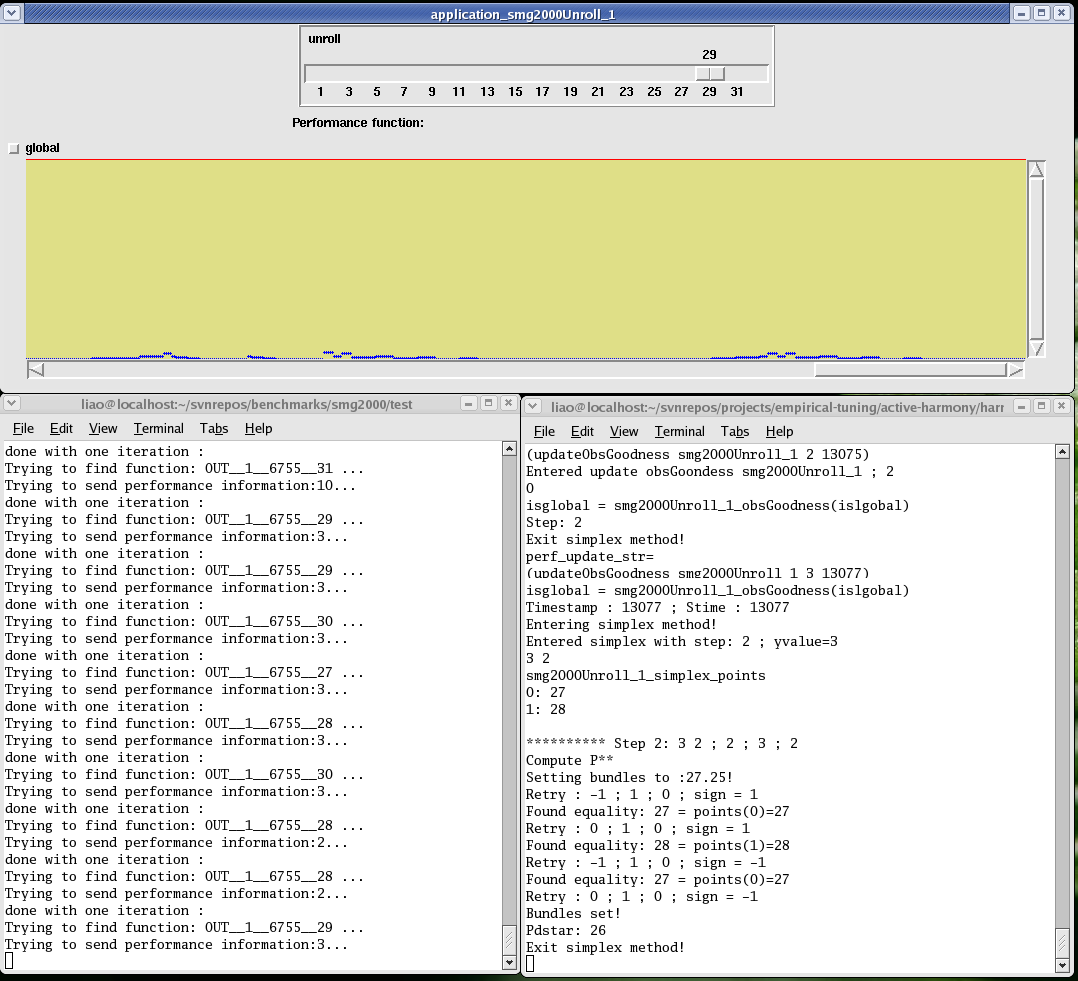
\includegraphics[width=0.8\textwidth]{activeHarmony2.png}
        \caption{Searching using Active Harmony}
        \label{fig:activeHarmony2}
\end{figure}

We have found that online/runtime search engines like the Active Harmony can be extremely expensive if the tuned kernel are invoked thousands of times. 
For SMG2000, it took hours to finish the tuning using a 120x120x120 input data set.
The major reason is that for each call of the kernel, a bidirectional communication between the client application and the server has to be finished. 
Another reason is that the current tuning process is embedded into the thousands of calls of the kernel so that points are always evaluated even when some of them have already been evaluated before. 



\input{userDirected}
\section{Summary}

   The work presented is ongoing work, and focused on the whole program empirical tuning
and the automation of all the required steps to make that work for realistic HPC applications
in C, C++, and Fortran.  
The work to has a few steps that are likely not so easy to fully
automate, namely the manipulation of the Makefiles and bash scripts that are required to support the empirical
tuning, but it is likely this can be simplified in the future.

The work presented is also immediately focused on providing an infrastructure for 
the empirical tuning and less on the empirical tuning of any specific applications.
SMG2000 was selected somewhat at random, since it is moderately large and 
we have demonstrated for many years that we can compile it easily with ROSE.


% just put it here temporarily
\commentout{
\section{Add Your Own Detector}

    Detectors written in Compass make direct use of ROSE and are 
designed to be copied and extended by users to develop their own 
detectors. We welcome the contribution of these detectors back to 
the ROSE team for inclusion into future releases of Compass;
full credit for all work will be provide to all authors.
Compass is an open source project using ROSE, an open source
compiler infrastructure.

  Guidelines for contributions:
\begin{itemize}
   \item Use any Compass detector and an example.
   \item provide the documentation about your detector.
   \item Use any features in ROSE to support your detector; AST, Control Flow graph,
    System dependence Graph, Call Graph, Class Hierarchy Graph, etc.
   \item Your detector should have no side-effects (on the AST).
\end{itemize}
}

\section{Design And Extensibility of Compass Detectors}

    The design of the detectors is intended to be simple
and with little required to be specified to build individual
detectors.  Of course some detectors may be non-trivial
(e.g. null pointer analysis, buffer overflow detectors, etc. 
(not yet provided in Compass)) the majority are simple.  All
detectors are meant to be side-effect free and are the subject
of separate research to independently provide automated 
combining (evaluation of multiple patterns in a single AST
traversal) and parallelization of the pattern evaluations on 
the AST.

\subsection{Input Parameter Specification}

    Parameters to all detectors are specified in an 
input parameter file (if required).  This permits numerous
knobs associated with different pattern detectors and separate
input files be specified for different software projects.

\subsection{Pattern Detection}
    Currently it is assumed that patterns will be detected as
part of a traversal of the AST.  See the ROSE Tutorial for example and 
general documentation on the different sorts of traversals possible 
within ROSE.

\subsection{Output Specification}

   Output of source position information specific to detected 
patterns are output in GNU standard source position formats.
See {\bf http://www.gnu.org/prep/standards/html\_node/Errors.html}
for more details on this format specification and now it is used
by external tools (e.g. emacs, etc.).









\bibliographystyle{plain}
\bibliography{minidb}
\listoffixmes
\end{document}

%
